
\documentclass[11pt, % The default document font size, options: 10pt, 11pt, 12pt
	oneside, % Two side (alternating margins) for binding by default, uncomment to switch to one side
	english, % ngerman for German
	onehalfspacing, % Single line spacing, alternatives: onehalfspacing or doublespacing
	%draft, % Uncomment to enable draft mode (no pictures, no links, overfull hboxes indicated)
	%nolistspacing, % If the document is onehalfspacing or doublespacing, uncomment this to set spacing in lists to single
	%liststotoc, % Uncomment to add the list of figures/tables/etc to the table of contents
	%toctotoc, % Uncomment to add the main table of contents to the table of contents
	parskip, % Uncomment to add space between paragraphs
	%nohyperref, % Uncomment to not load the hyperref package
	%headsepline, % Uncomment to get a line under the header
	%chapterinoneline, % Uncomment to place the chapter title next to the number on one line
	%consistentlayout, % Uncomment to change the layout of the declaration, abstract and acknowledgements pages to match the default layout
	]{article} % The class file specifying the document structure
\usepackage[a4paper, total={5.5in, 8in}]{geometry}
\setcounter{tocdepth}{2}
\usepackage{amsmath,amsfonts,amsthm,amssymb,mathtools}
% \numberwithin{equation}{section}
\usepackage[T1]{fontenc}
\usepackage{mlmodern}
\usepackage{xfrac}
\usepackage[makeroom]{cancel}
\usepackage{mathtools}
\usepackage{bookmark}
\usepackage{enumitem}
\usepackage{xcolor}
\usepackage{varwidth}
\usepackage{varwidth}
\usepackage{etoolbox}
\usepackage{nameref}
\usepackage{multicol,array}
\usepackage{import}
\usepackage{pdfpages}
\usepackage{todonotes}
\usepackage{booktabs}
\usepackage{tikz}
\usetikzlibrary{calc,arrows.meta}

% \setlength{\baselineskip}{6pt plus 2pt minus 1pt}
\setlength{\parskip}{6pt plus 2pt minus 1pt}
\setlength{\parindent}{12pt}

\usepackage{floatrow}
% \floatsetup[figure]{capposition=top}

\newtheorem{theorem}{Theorem}
\newtheorem{proposition}{Proposition}
\newtheorem{corollary}{Corollary}
\newtheorem{lemma}{Lemma}
\theoremstyle{definition}
\newtheorem{definition}{Definition}
\AtBeginEnvironment{definition}{%
  \pushQED{\qed}\renewcommand{\qedsymbol}{$\diamond$}%
}
\AtEndEnvironment{definition}{\popQED\enddefinition}
\newtheorem{remark}{Remark}

\newtheorem{example}{Example}
\AtBeginEnvironment{example}{%
  \pushQED{\qed}\renewcommand{\qedsymbol}{$\triangle$}%
}
\AtEndEnvironment{example}{\popQED\endexample}

\setcounter{tocdepth}{2}

% COLOR DEFINITION

% Link Colors
\hypersetup{
  colorlinks   = true, %Colours links instead of ugly boxes
  urlcolor     = blue, %Colour for external hyperlinks
  linkcolor    = blue, %Colour of internal links
  citecolor   = red %Colour of citations
}


\title{\Huge{Foundations of Data Science}}
\author{Ralf Blöchlinger}
\date{Fall 2024}


\graphicspath{ {.} }


\begin{document}
\maketitle

\tableofcontents

\newpage




\subsubsection*{Definition of Machine Learning}

A computer program is said to learn from experience $E$ with respect to some class of tasks $T$ and performance measure $P$, if its performance at tasks in $T$, as measured by $P$, improves with experience $E$.\footnote{E.g., $E$ is training data set consisting of faces, $T$ is to put boxes around faces, $P$ is number of correctly identified faces.}

\begin{center}
	Learning = Representation + Evaluation + Optimisation
\end{center}
\begin{itemize}
	\item Representation: Hypothesis space, which models to consider
	\item Evaluation: Objective function
	\item Optimization: Search method for optimizing objective function
\end{itemize}

\subsubsection*{Perceptron}
\begin{equation*}
	\operatorname{sign}(\boldsymbol{w} \cdot \mathbf{x})= \begin{cases}+1 & \text { if } \boldsymbol{w} \cdot \mathbf{x} \geq 0 \\ -1 & \text { otherwise }\end{cases}
\end{equation*}

Algorithm: Initialize $\mathbf{w} = 0$. Repeat until convergence, for $t = 1, ..., n$:
\begin{enumerate}
	\item Compute prediction: $y^{\prime}=\operatorname{sign}\left(\mathbf{x}_t \cdot w\right)$
	\item Update parameters:
	\begin{itemize}
		\item If $y^{\prime} \neq y_t \text { then } \mathbf{w}:=\mathbf{w}+y_t \mathbf{x}_t$\footnote{If $y' = 1, y_t = -1$, we want to make $\mathbf{w} \cdot \mathbf{x}_t$ smaller. Note that $\mathbf{w'} \cdot \mathbf{x}_t = \mathbf{w} \mathbf{x}_t + y  \mathbf{x}_t^\top  \mathbf{x}_t < \mathbf{w} \cdot  \mathbf{x}_t$.}
		\item else, leave $\mathbf{w}$ unchanged
	\end{itemize}
\end{enumerate}


\section{Linear Regression}

Linear model:
\begin{equation*}
	y=w_0+x_1 w_1+\cdots+x_D w_D+\epsilon
\end{equation*}
where $y$ is a $N \times 1$ vector.

Estimate $\hat{\mathbf{w}}$ by optimizing \emph{Least Squares objective function}:
\begin{equation*}
	\arg \min_\mathbf{w}  \frac{1}{2 N} \sum_{i=1}^N\left(\mathbf{x}_i^{\top} \mathbf{w}-y_i\right)^2=\frac{1}{2 N}(\mathbf{X} \mathbf{w}-\mathbf{y})^{\top}(\mathbf{X} \mathbf{w}-\mathbf{y})
\end{equation*}
where we usually include a vector of ones in the matrix $\mathbf{X}$.

\begin{itemize}
	\item Simple linear regression with one predictor:
	\begin{equation*}
		w_0=\bar{y}-w_1 \cdot \bar{x}; \; w_1=\frac{\widehat{\operatorname{cov}}(x, y)}{\widehat{\operatorname{var}}(x)}
	\end{equation*}

	\item General solution:
	\begin{equation*}
		\mathbf{w}=\left(\mathbf{X}^{\top} \mathbf{X}\right)^{-1} \mathbf{X}^{\top} \mathbf{y}
	\end{equation*}
	\begin{itemize}
		\item Complexity: $O(D^2N + D^3)$
		\item $\mathbf{X}^T \mathbf{X}$ invertible if full rank, i.e., rank is $D+1$ and $N > D$
	\end{itemize}
	\item Predictions: $\hat{\mathbf{y}} = \mathbf{X} {\mathbf{w}}$; for a single observation $\hat{y} = \mathbf{x} \cdot \mathbf{w}$
\end{itemize}


\subsubsection*{Huber Loss}

Due to square, OLS is non-robust. Alternative: Huber-Loss function which is equal to OLS for small deviations and is an absolute value loss for larger values.

\begin{definition}
	Given arbitrary but fixed parameters $\lambda, \mu \in \mathbb{R}$ with $\lambda, \mu>0$, the \textbf{Huber loss} is given by the function $h_{\lambda, \mu}: \mathbb{R} \mapsto \mathbb{R}$ such that
$$
h_{\lambda, \mu}(z)= \begin{cases}\lambda\left(|z|-\frac{\lambda}{4 \mu}\right), & \text { if }|z| \geq \frac{\lambda}{2 \mu} \\ \mu z^2, & \text { otherwise }\end{cases}
$$
\end{definition}

Another alternative involves using the absolute error instead of the squared error. This problem cannot be solved in closed-form as the absolute value function is not differentiable everywhere.


\subsection{Basis Expansion}

Idea: Capture non-linearities in linear regression by including transformations of feature space.

\begin{itemize}
	\item Example: Quadratic model with 2 predictors
	\begin{equation*}
		\psi(\mathbf{x})=\left[1, x_1, x_2, x_1^2, x_2^2, x_1 x_2\right]^{\top}
	\end{equation*}
	\item degree $d$ polynomial, $D$ dimensions $\implies O(D^d)$ features
	\item Computational cost dominated by dot product
	\item Can reduce cost by using kernels. For some expansion $\phi$ a kernel function computes the dot product efficiently\footnote{The idea is to directly compute the kernel function in the original space instead of first manually creating the expansion and then computing the dot product of this expansion (i.e., in the high-dimensional space induced by the expansion). For instance, for $\kappa_{\text {poly }}\left(\mathbf{x}^{\prime}, \mathbf{x}\right)=\left(\mathbf{x} \cdot \mathbf{x}^{\prime}\right)^d$, we can calculate this in expansion form as:
	\begin{equation*}
		\left(\mathbf{x} \cdot \mathbf{x}^{\prime}\right)^d=\sum_{n_i \geq 0, \sum_i n_i=d} \underbrace{\sqrt{C\left(d ; n_1, \ldots, n_D\right)} x_1^{n_1} \cdots x_D^{n_D}}_{\text {one row in } \phi_{\text {odlv }}(\mathbf{x})} \underbrace{\sqrt{C\left(d ; n_1, \ldots, n_D\right)}\left(x_1^{\prime}\right)^{n_1} \cdots\left(x_D^{\prime}\right)^{n_D}}_{\text {one row in } \phi_{\text {olly }}\left(\mathbf{x}^{\prime}\right)}
	\end{equation*}
	which is $O(D^d)$. Instead directly computing $\left(\mathbf{x} \cdot \mathbf{x}^{\prime}\right)^d$ is $O(D + \log d)$. For the RBF kernel, the expansion involves a projection onto an infinte dimensional space, so using an expansion is unfeasible. For some kernels, we are directly interested in using the kernels as features, as we compare our data points to some fixed vectors. For other expansions, such as polynomial expansions, whether we can use kernels depends on the way in which the polynomial expansion enters the objective function or solution (i.e., whether it occurs in form of a dot product.)
	 }
	\begin{equation*}
		\kappa\left(\mathbf{x}^{\prime}, \mathbf{x}\right): \mathcal{X} \times \mathcal{X} \rightarrow \mathbb{R}, \quad \kappa\left(\mathbf{x}^{\prime}, \mathbf{x}\right)=\phi\left(\mathbf{x}^{\prime}\right) \cdot \phi(\mathbf{x})
	\end{equation*}
	\item Polynomial Kernel: $\kappa_{\text {poly }}\left(\mathbf{x}^{\prime}, \mathbf{x}\right)=\left(\mathbf{x} \cdot \mathbf{x}^{\prime}+\theta\right)^d$
	\item Radial Basis Function kernel: $\kappa_{\mathrm{RBF}}\left(\mathbf{x}^{\prime}, \mathbf{x}\right)=\exp \left(-\gamma\left\|\mathbf{x}-\mathbf{x}^{\prime}\right\|^2\right)$.
	\begin{itemize}
		\item Hyperparameters: center and width. Narrow kernels (large $\gamma$) increase overfitting risk.
		\item Dissimilarity measure, $\kappa$ close to 1 if points are close.
	\end{itemize}
\end{itemize}

We use kernels as features. For some kernel basis expansion, the linear model is
\begin{equation*}
	\boldsymbol{y}=w_0+w_1 \kappa\left(\mu_1, \mathbf{x}\right)+\cdots+w_M \kappa\left(\mu_M, \mathbf{x}\right)+\epsilon=\mathbf{w} \cdot \boldsymbol{\psi}(\mathbf{x})+\epsilon
\end{equation*}
where centers $\mu_i$ are hyperparameters.

Choosing $\gamma$:
\begin{itemize}
	\item High $\gamma$, narrow width: overfitting, can be reduced with more data
	\item Low $\gamma$, wide width: underfitting
	\item \emph{Curse of dimensionality}: In  high-dimensional space, we easily underfit as Euclidian distances between all data points is large and similar. Recall that kernels measure similarity. Therefore, kernels lose power in large dimensions. Dataset needs to be exponentially large in dimension or underfitting occurs.
\end{itemize}

\emph{Radial basis kernels are universal} but too powerful (overfitting) and computationally expensive.


\section{Learning Curves, Validation, Feature Selection}

\subsection{Learning Curves}

Fundamental Goal of ML: Generalizing beyond the training set.

\begin{itemize}
	\item No free lunch theorem: Impossible to beat random guessing over all possible functions one can learn
	\item Context knowledge can limit which functions are reasonable
\end{itemize}

\subsubsection*{Bias-Variance Tradeoff:}
\begin{equation*}
	\text{Generalisation error = bias + variance}
\end{equation*}
\begin{itemize}
	\item Bias: consistently learn wrong thing $\to$ Underfitting
	\item Variance: Learn random things irrespetive of true signal $\to$ Overfitting
	\item Averaging high variance models can reduce overfitting $\to$ \emph{ensemble models}
\end{itemize}

\subsubsection*{Learning curves:}
\begin{enumerate}
	\item Split data into training and testing set.
	\item Train on increasing sizes of data. \item Plot train and test error as function of training data size
	\item If test error > train error, but decreasing in data size, more data would be useful.
	\item If test error and train error are close, more data would not be useful. Potentially a good-working model or underfitting.
\end{enumerate}

\subsection{Regularisation}

Three ways to avoid overfitting:
\begin{enumerate}
	\item Regularisation
	\item Cross-validation
	\item Statistical signifiance tests before adding new features (e..g, $\chi^2$-test)
\end{enumerate}

Idea of regularisation: add penalty term for model parameters.

\subsubsection*{Ridge Regression}

\begin{equation*}
	\mathcal{L}_{\text {ridge }}(\mathbf{w})=(\mathbf{X w}-\mathbf{y})^{\top}(\mathbf{X} \mathbf{w}-\mathbf{y})+\lambda \sum_{i=1}^D w_i^2
\end{equation*}
$\ell_2$-regularisation on weights.

\begin{itemize}
	\item Penalty on all coefficients but intercept (intercept is output translation, not model complexity)
	\item Standardise input to avoid dependency on scaling $x' = (x- \mu) / \sigma$
	\item Additionally demean $\mathbf{y}$ s.t. $w_0 = 0$. Can then be rewritten as
	$$\mathcal{L}_{\text {ridge }}(\mathbf{w})=(\mathbf{X w}-\mathbf{y})^{\top}(\mathbf{X} \mathbf{w}-\mathbf{y}) +\lambda \mathbf{w}^{\top} \mathbf{w}$$
	\item Closed-form solution:
	\begin{equation*}
		\mathbf{w}_{\text {ridge }}=\left(\mathbf{X}^{\top} \mathbf{X}+\lambda \mathbf{I}_D\right)^{-1} \mathbf{X}^{\top} \mathbf{y}
	\end{equation*}
	\item Note: perturbed matrix, $\mathbf{X}^T \mathbf{X}$ is psd, so $\mathbf{X}^{\top} \mathbf{X}+\lambda \mathbf{I}_D$ is pd and invertible
	\item Can rewrite as Lagrangian: (Inverse relation between $R$ and $\lambda$)
	\begin{equation*}
		\min (\mathbf{X w}-\mathbf{y})^{\top}(\mathbf{X w}-\mathbf{y})  \text { subject to }  \mathbf{w}^{\top} \mathbf{w} \leq R
	\end{equation*}
\end{itemize}

\subsubsection*{Least Absolute Shrinkage and Selection Operator}

\begin{equation*}
	\mathcal{L}_{\text {lasso }}(\mathbf{w})=(\mathbf{X w}-\mathbf{y})^{\top}(\mathbf{X w}-\mathbf{y})+\lambda \sum_{i=1}^D\left|w_i\right|
\end{equation*}
\begin{itemize}
	\item $\ell_1$ penalty
	\item No closed form solution
	\item Contout or objective function is mix between oval and diamond when viewing level sets. Solutions tend to be on corner of diamond restriction on $|\mathbf{w}|$ (Figure \ref{fig.lasso}). We therefore have feature selection as some coefficients are often $0$ $\to$ \emph{sparse models}
\end{itemize}

\begin{figure}[ht!]
    \caption{Left: Contour line of objective function. Right: Contour line of MSE with LASSO penalisation term in dashed lines.}
    \label{fig.lasso}
    \begin{center}
        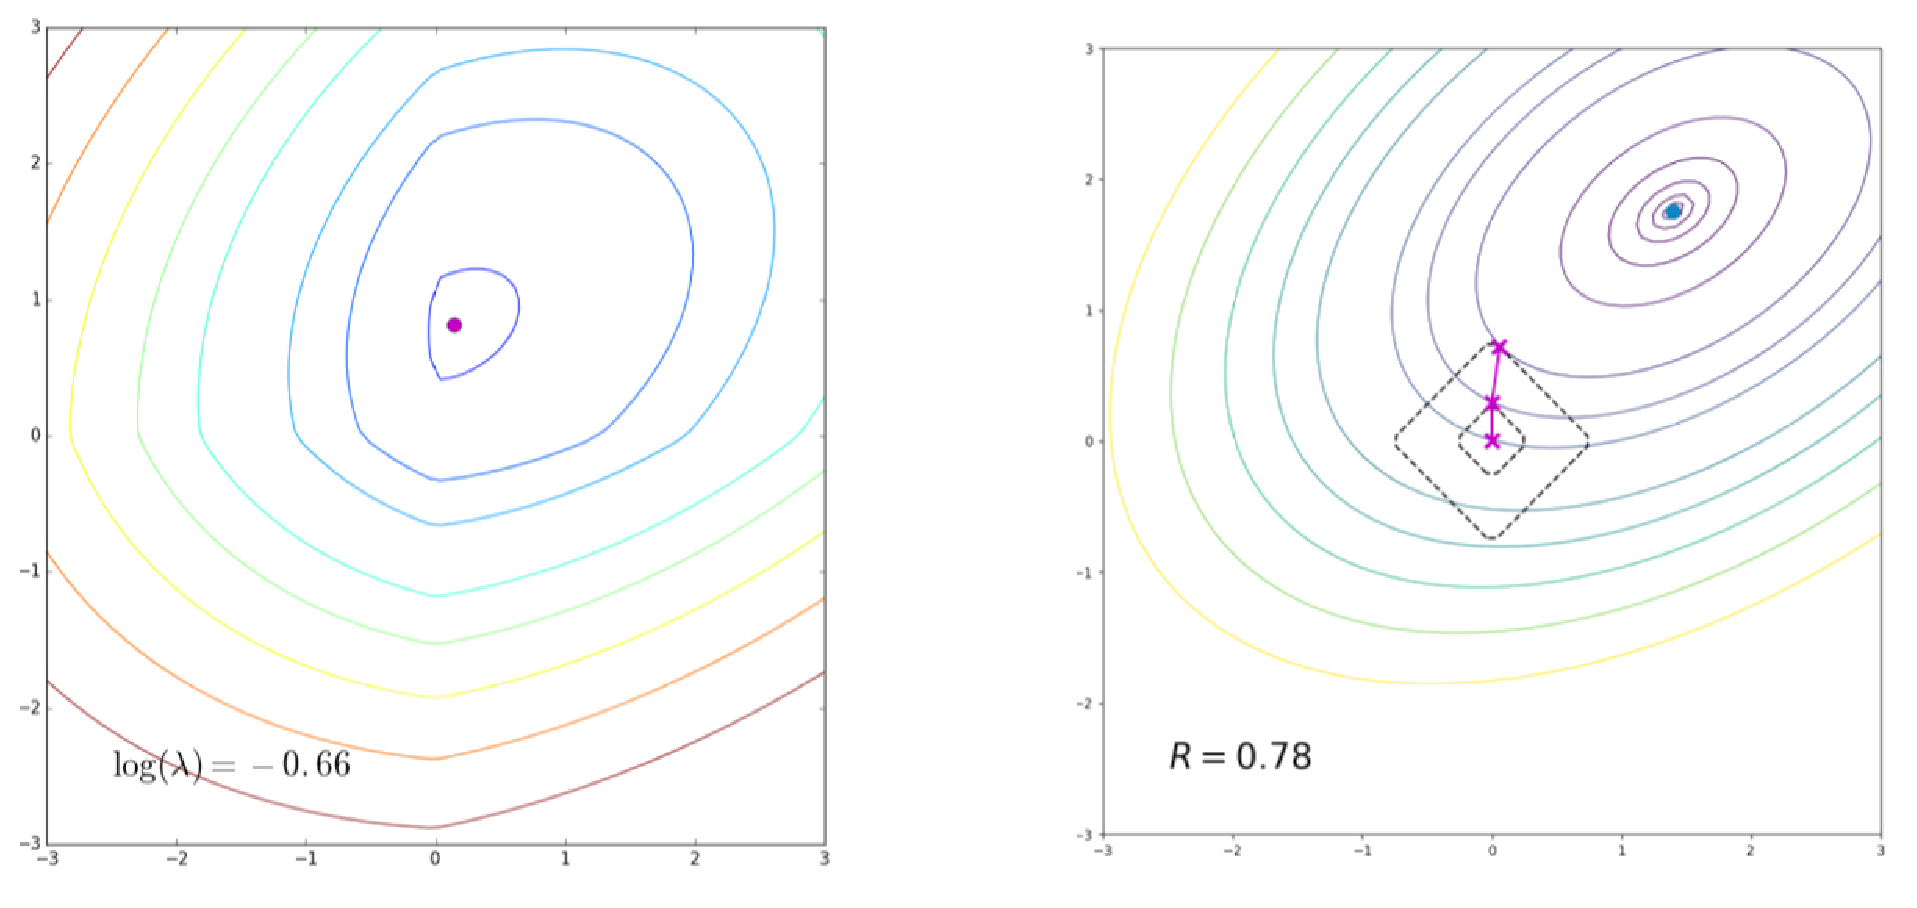
\includegraphics[width = 0.8\textwidth]{lasso_cont.pdf}
    \end{center}
\end{figure}


\subsection{Validation}


Suppose we want to choose the optimal value of one hyperparemter.

\begin{enumerate}
	\item Divide the data into parts: training, validation
	\begin{itemize}
		\item Testing data is separate from both training and validation data
	\end{itemize}
	\item For each value of $\lambda$, train model using the training set and evaluate on the validation set
	\item Pick the value of $\lambda$ that minimises the validation error\footnote{Often U-shaped curve. E.g., LASSO with low $\lambda$ overfits, with high $\lambda$ underfits}
\end{enumerate}

Multiple hyperparameters: \textbf{Grid search}

\begin{itemize}
	\item Iterate over all possible combinations of hyper-parameter values $D_1 \times \cdots \times D_k$
	\item Perform cross-validation for each such combination
\end{itemize}

\subsubsection*{Cross Validation}

When data is scarce, instead of splitting as training and validation, divide data into $K$ folds (parts):
\begin{itemize}
	\item Use $K-1$ folds for training and 1 fold as validation
	\item Validation error for fixed hyper-parameter values: average over all runs (i.e., train with same hyper-parameter on all $K$ possible combinations of $K-1$ folds and calculate average of error on each validation fold.)
	\item When $K = N$, LOOCV
\end{itemize}


\subsection{Feature Selection}

Goal: Given large feature set, select relevant features for model.

\begin{itemize}
	\item Data often contains redundant or irrelevant features, e.g., due to strong correlations or not predictive power
	\item Selecting only relevant features reduces overfitting risk, avoids curse of dimensionality, yields simpler models, reduces training time
\end{itemize}

Each feature selection method usually consists of two components:
\begin{enumerate}
	\item Search technique for subsets of given features
	\item Evaluation measure to rank different subsets
\end{enumerate}
Approaches:
\begin{enumerate}

	\item \textbf{Wrapper methods}: train new model for each subsets.
	\begin{itemize}
		\item Exhaustive search unfeasible as $2^n$ subsets of $n$ features
		\item Instead, e.g., forward stepwise selection\footnote{For $D$ features, for each $1 \leq i \leq D$: What is best $i$ feature model, given previously selected $i-1, i-2, \dots$ features. Note: $O(D^2)$ models to train. Can be implemented as same complexity as one model for linear regression.}
	\end{itemize}
	\item \textbf{Filter methods}: proxy measure as score instead of test error
	\begin{itemize}
		\item E.g., calculate correlation or mutual information\footnote{
			Mutual information for two RVs $X,Y$ is given by $I(X, Y)=\sum_x \sum_y p(X=x, Y=y) \cdot \log \frac{p(X=x, Y=y)}{p(X=x) \cdot p(Y=y)}$. Approximate by bucketizing features into discrete bins and counting fraction in training set for each bin.
		} between features and target
	\end{itemize}
	\item \textbf{Embedded methods}: Perform feature selection while constructing model
	\begin{itemize}
		\item E.g., LASSO or elastic net regularisation
	\end{itemize}
\end{enumerate}


\section{Optimization}

Two general approaches:
\begin{enumerate}
	\item Convex optimization problem $\to$ use blackbox solvers
	\item Gradient-based optimization methods\footnote{Not blackbox, optimization hyperparameters affect performance}
\end{enumerate}

\subsection{MLE}

Alternative view for ML: explicitly formulate the deviation (or uncertainty) from the model using probability theoretic notions.

\begin{itemize}
	\item Given: Observations $x_1, \ldots, x_N$ iid drawn from distr $p$
	\item Likelihood of observing $x_1, \ldots, x_N \approx$ probability of making these observations assuming they are generated according to $p$
	\begin{itemize}
		\item $p$ has a parametric form, e.g., depends on the parameter vector $\boldsymbol{\theta}$
		\item $p\left(x_1, \ldots, x_N \mid \boldsymbol{\theta}\right)$ : joint probability distr. of observations given $\boldsymbol{\theta}$
	\end{itemize}
	\item \emph{Maximum Likelihood Principle}: Pick parameter $\boldsymbol{\theta}$ that maximises the likelihood
	$$
	\boldsymbol{\theta}^*=\underset{\boldsymbol{\theta}}{\operatorname{argmax}} \; p\left(x_1, \ldots, x_N \mid \boldsymbol{\theta}\right)
	$$
	\item Since the observations are i.i.d.: $p\left(x_1, \ldots, x_N \mid \theta\right)=\prod_{i=1}^N p\left(x_i \mid \theta\right)$
\end{itemize}


\subsubsection*{MLE for Linear Regression}

Assumption: Give $\mathbf{x}$ and $\mathbf{w}$, $y$  is normal with mean $\mathbf{w}^{\top} \mathbf{x}$ and variance $\sigma^2$
$$
p(y \mid \mathbf{w}, \mathbf{x})=\mathcal{N}\left(\mathbf{w}^{\top} \mathbf{x}, \sigma^2\right)=\mathbf{w}^{\top} \mathbf{x}+\mathcal{N}\left(0, \sigma^2\right)
$$
Equivalently, $\epsilon \sim \mathcal{N}\left(0, \sigma^2\right)$. We assume $\mathbf{X}$ to be fixed (non-random).

\begin{equation*}
	\begin{aligned}
		p(\mathbf{y} \mid \mathbf{X}, \mathbf{w}, \sigma)=\left(\frac{1}{2 \pi \sigma^2}\right)^{N / 2} \exp \left(-\frac{1}{2 \sigma^2}(\mathbf{X} \mathbf{w}-\mathbf{y})^{\top}(\mathbf{X} \mathbf{w}-\mathbf{y})\right) \\
		\operatorname{NLL}(\mathbf{y} \mid \mathbf{X}, \mathbf{w}, \sigma)=\frac{1}{2 \sigma^2}(\mathbf{X w}-\mathbf{y})^{\top}(\mathbf{X} \mathbf{w}-\mathbf{y})+\frac{N}{2} \log \left(2 \pi \sigma^2\right)
	\end{aligned}
\end{equation*}
\begin{itemize}
	\item Maximizing likelihood is equivalent to maximizing log-likelihood (or min $NLL$) as log is strongly montone.
	\item Objective function identical to Least Squares up to additive and multiplicative constant.
	\item Same estimator for MLE and OLS
	\item Can create confidence intervals for new predictions $y_{\text {new }} \sim \widehat{y}_{\text {new }}+\mathcal{N}\left(0, \sigma_{\text {ML }}^2\right)$.\footnote{Note that this is imprecise as we estimate the coefficients and thus need to account for this additional uncertainty.}
\end{itemize}

\subsubsection*{Robust Regression}

Use noise distribution with fatter tails, e.g., Laplacian.
\begin{align*}
	p\left(y_1, \ldots, y_N \mid \mathbf{x}_1, \ldots, \mathbf{x}_N, \mathbf{w}, b\right)=\prod_{i=1}^N \frac{1}{2 b} \exp \left(-\frac{\left|y_i-\mathbf{w}^{\top} \mathbf{x}_i\right|}{b}\right) \\
	\operatorname{NLL}(\mathbf{y} \mid \mathbf{X}, \mathbf{w}, b)=\frac{1}{b} \sum_{i=1}^N\left|y_i-\mathbf{w}^{\top} \mathbf{x}_i\right|+N \log (2 b)
\end{align*}

\begin{itemize}
	\item Identical to linear regression with absolute value objective function instead of squared sum of residuals $\to$ robust to outliers
	\item No closed form solution, not differentiable anywhere
	\item Can be solved as convex linear optimization problem
\end{itemize}


\subsection{Convex Optimization}

\begin{definition}
	A set $C \subseteq \mathbb{R}^D$ is convex if for any $\mathbf{x}, \mathbf{y} \in C \text { and } \lambda \in[0,1]$, it holds $\lambda \mathbf{x}+(1-\lambda) \mathbf{y} \in C$
\end{definition}

\begin{definition}
	A function $f: \mathbb{R}^D \rightarrow \mathbb{R}$ defined on a convex domain is convex if: for all $\mathbf{x}, \mathbf{y} \in \mathbb{R}^D$ where $f$ is defined and $0 \leq \lambda \leq 1$,
	$$
	f(\lambda \cdot \mathbf{x}+(1-\lambda) \cdot \mathbf{y}) \leq \lambda \cdot f(\mathbf{x})+(1-\lambda) \cdot f(\mathbf{y})
	$$
\end{definition}

Examples of convex functions:
\begin{itemize}
	\item Affine functions: $f(\mathbf{x})=\mathbf{b}^{\top} \mathbf{x}+c$
	\item Quadratic functions: $f(\mathbf{x})=1 / 2 \cdot \mathbf{x}^{\top} \mathbf{A} \mathbf{x}+\mathbf{b}^{\top} \mathbf{x}+c$, where $\mathbf{A}$ is symmetric positive semidefinite
	\item Nonnegative weighted sums of convex functions: Given convex functions $f_1, \ldots, f_n$ and $w_1, \ldots, w_n \in \mathbb{R}_{\geq 0}$, the following is a convex function $f(\mathbf{x})=\sum_{i=1}^n w_i \cdot f_i(\mathbf{x})$
	\item Norms: $\|\cdot\|_p$ except $p=0$
\end{itemize}

\subsubsection*{Convex optimization problem}

Given convex functions $f, g_1, \ldots, g_m$ and affine functions $h_1, \ldots h_{n}$:
$$
\begin{aligned}
& \text {minimise } f(\mathbf{x}) \\
& \text {subject to } g_i(\mathbf{x}) \leq 0 \quad i \in[m] \\
& h_j(\mathbf{x})=0 \quad j \in[n]
\end{aligned}
$$
Goal: When $S$ is set of feasible functional values, want to find optimal value $v^* = \min S$ and optimal point $\mathbf{x}^* = \arg \min S$.\footnote{For infeasible problems, we set $v^* = \infty$, for unbounded problems $v^* = -\infty$.}

\begin{theorem}
	For any convex optimisation problem, all locally optimal points are globally optimal.
\end{theorem}

\begin{proof}
	By contradiction, asumme $x$ local optimum, $y$ global optimum with $f(y) < f(x)$. Since local optimum $\exists B$ s.t. $f(x) < f(x')$ for any feasible $x'$ with $||x-x'||_2 < B$. Choose $z = \lambda y + (1-\lambda) x$ and $\lambda = B /(2 ||x-y||_2)$. Then $||x-z||_2 < B$ and $f(z) \leq \lambda f(y) + (1-\lambda) f(x) < f(x)$ contradicting that $x$ is a local optimum.
\end{proof}

Common examples:
\begin{itemize}
	\item Linear program:\footnote{Space of feasible solutions is polytope defined by intersection of half-spaces of constraints. Solution is always at an edge (\emph{vertex}) of polytope. In particular, we want to find the vertex which projected onto $-\mathbf{c}$ gives the longest vector.}
	\begin{equation*}
		\begin{array}{r}
			\text { minimize } \mathbf{c}^{\top} \mathbf{x}+d \\
			\text { subject to } \mathbf{A} \mathbf{x} \leq \mathbf{e} \\
			\mathbf{B} \mathbf{x}=\mathbf{f}
		\end{array}
	\end{equation*}
	\item Quadratically Constrained Quadratic Programming:
	\begin{equation*}
		\begin{aligned}
			& \text { minimize } \frac{1}{2} \mathbf{x}^{\top} \mathbf{B} \mathbf{x}+\mathbf{c}^{\top} \mathbf{x}+d \\
			& \text { subject to } \frac{1}{2} \mathbf{x}^{\top} \mathbf{Q}_i \mathbf{x}+\mathbf{r}_i^{\top} \mathbf{x}+s_i \leq 0 \; i \in[m] \\
			& \mathbf{A} \mathbf{x}=\mathbf{b}
		\end{aligned}
	\end{equation*}
\end{itemize}
No closed form solutions but efficient algortihms (polynomial time) exist.

Showing that a linear program is equivalent to some maximization problem:
\begin{enumerate}
	\item Show that there exists some solution to linear program
	\item Show that the optimal solution for lin prog coincides with solution of mathematical optimization problem
\end{enumerate}

Linear regression is quadratic convex program. Lasso can be rephrased as quadratic program with linear constraints.

\subsection{Gradient Descent}

\subsubsection*{Geometry of Gradient and Hessian}

\begin{theorem}
	If a function $f$ is differentiable, the gradient of $f$ at a point is either zero or perpendicular to the contour line of $f$ at that point.
\end{theorem}

\begin{itemize}
	\item Intuition: Along a contour line the functional value does not change thus $\nabla_\mathbf{x} f \cdot \mathbf{v} = 0$ if $\mathbf{v}$ is vector tangent to contour line.
\end{itemize}

\begin{theorem}
	The gradient $\nabla_{\mathbf{v}} f$ of a function $f$ points in the direction of steepest ascent.
\end{theorem}

\begin{itemize}
	\item Consider the directional derivative:
	\begin{equation*}
		\nabla_{\mathbf{v}} f(\mathbf{a})=\lim _{h \rightarrow 0} \frac{f(\mathbf{a}+h \mathbf{v})-f(\mathbf{a})}{h}=\nabla f(\mathbf{a}) \cdot \mathbf{v}
	\end{equation*}
	\item We want to find the unit vector maximizing this quantitiy, from dot product definition,
	\begin{equation*}
		\nabla f(\mathbf{a}) \cdot \mathbf{v}=\|\nabla f(\mathbf{a})\|\|\mathbf{v}\| \cos \theta.
	\end{equation*}
	which is maximized for $\theta = 0$, i.e., $\mathbf{v}$ points into direction of gradient.
\end{itemize}

\emph{Hessian} is symmetric if all second-order derivatives exist and are continuous. Captures curvature of surface. A saddle point is a minimum if all eigenvalues of $\mathbf{H}$ at $\mathbf{x}^*$ are positive.

\subsubsection*{Gradient Descent Algorithm}

At each point $t$, update weights using
\begin{equation*}
	\mathbf{w}_{t+1}=\mathbf{w}_t-\eta_t \mathbf{g}_t=\mathbf{w}_t-\eta_t \nabla f\left(\mathbf{w}_t\right),
\end{equation*}
where $\eta > 0$ is learning rate.

Gradient descent can also be used if closed-form solutions exist. E.g., OLS closed-form is $O(ND^2 + D^3)$, each gradient step
\begin{equation*}
	\nabla_{\mathbf{w}} \mathcal{L}=2\left(\mathbf{X}^{\top} \mathbf{X} \mathbf{w}-\mathbf{X}^{\top} \mathbf{y}\right) = 2 \mathbf{X}^{\top} \left( \mathbf{X} \mathbf{w}- \mathbf{y}\right)
\end{equation*}
is $O(ND)$.\footnote{First compute $X w - y$.} If number of iterations $K < D$, gradient descent is more efficient.

Choosing step size:
\begin{itemize}
	\item Idea: smaller steps the closer to optimum
	\item Constant step size: $\eta_t=\mathrm{c}$
	\item Decaying step size: $\eta_t=\mathrm{c} / t$ for constant $c$. Another common decay rate: $\frac{1}{\sqrt{t}}$
	\item Backtracking line search:
	\begin{enumerate}
		\item Start with $c/t$
		\item Check if the function value decreases after the weight update, i.e., if $f\left(\mathbf{w}_t-\right.$ $\left.\eta_t \boldsymbol{\nabla} f\left(\mathbf{w}_t\right)\right)<f\left(\mathbf{w}_t\right)$ holds.
		\item If the decrease condition is not met, multiply $\eta_t$ by a decaying factor to decrease step size
		\item Repeat the previous two steps until the decrease condition is met.
	\end{enumerate}
\end{itemize}

Convergence tests:
\begin{itemize}
	\item Fixed number of iterations
	\item Small change in the function value: Terminate if $\left|f\left(\mathbf{w}_{t+1}\right)-f\left(\mathbf{w}_t\right)\right| \leq \epsilon_1$
	\item Small change in the parameter values: Terminate if $\left\|\mathbf{w}_{t+1}-\mathbf{w}_t\right\|_2 \leq \epsilon_2$
\end{itemize}

\subsubsection*{Stochastic Gradient Descent}
Gradient is expensive since we need to take average of gradient of objective function for each observation. Instead, only take one data point (\emph{online learning}) or a mini-batch to compute gradient.

Example: For Ridge,
$$
\nabla_{\mathbf{w}} \mathcal{L}=\frac{1}{N} \sum_{i=1}^N \nabla_{\mathbf{w}} \ell\left(\mathbf{w} ; \mathbf{x}_i, y_i\right)+\lambda \nabla_{\mathbf{w}} \mathcal{R}(\mathbf{w})
$$

Pick a random datapoint $\left(\mathbf{x}_i, y_i\right)$ and evaluate $\mathbf{g}_i=\nabla_{\mathbf{w}} \ell\left(\mathbf{w} ; \mathbf{x}_i, y_i\right)$. Then,
$$
\mathbb{E}\left[\mathbf{g}_i\right]=\frac{1}{N} \sum_{i=1}^N \nabla_{\mathbf{w}} \ell\left(\mathbf{w} ; \mathbf{x}_i, y_i\right)
$$
In expectation $\mathbf{g}_i$ points in the same direction as the entire gradient (except for the regularisation term).\footnote{Actually, it also holds for the regularisation term. However, if one were to use a sum instead of mean in the lossfunction, one should scale up the single function gradient by a factor $N$ to ensure that the relative scale is correct. The regularisation term usually does not depend on the specific observation chosen.}

\begin{itemize}
	\item SGD will jump around a lot more, more variance
	\item In practice, mini-batch gradient descent performs far better
\end{itemize}

\subsubsection*{Subgradient Descent}

Consider LASSO.
\begin{itemize}
	\item Due to absolute value function, this is not differentiable everywhere $\to$ problem for gradient descent.
	\item Non-unique slope but can pick one possible slope value
\end{itemize}

\begin{definition}[Sub-Derivatives and Sub-Gradients]
	A sub-derivative of a univariate convex function $f$ at a point $x_0$ is a scalar $g$ such that
	$$
	f(x) \geq f\left(x_0\right)+g \cdot\left(x-x_0\right) \quad \text { for all } x .
	$$

	A sub-gradient of a multivariate convex function $f$ at a point $\mathbf{x}_0$ is a vector $\mathbf{g}$ such that
	$$
	f(\mathbf{x}) \geq f\left(\mathbf{x}_0\right)+\mathbf{g}^{\boldsymbol{\top}}\left(\mathbf{x}-\mathbf{x}_0\right) \quad \text { for all } \mathbf{x} .
	$$
\end{definition}

We thus replace the gradient (in gradient descent) with a subgradient at a point where the function is not differentiable.

\subsubsection*{Constrained convex optimisation and gradient descent}

Suppose we have $\min f(\mathbf{x})$ subject to additional constraints $\mathbf{w}_C \in C$. We can use projected gradient descent.

$$
\begin{aligned}
\text{Gradient step: } \; &\mathbf{z}_{t+1}  =\mathbf{w}_t-\eta_t \nabla f\left(\mathbf{w}_t\right) \\
\text{Projection step: } \; &\mathbf{w}_{t+1}  =\underset{\mathbf{w}_C \in C}{\operatorname{argmin}}\left\|\mathbf{z}_{t+1}-\mathbf{w}_C\right\|
\end{aligned}
$$

I.e., we first calculate the gradient while ignoring constraints and then project our updated value back into the set of feasible values $C$.\footnote{Ridge using the penalty term objective is a more efficient approach than using it in ``Lagrange'' form as we can compute the gradient directly without the projection step.}

\subsubsection*{Newton's Method}

Newton's method is a second order method which uses not only the first but also the second derivative (or Hessian in multivariate case). In some cases, this can lead to faster convergence. Instead of fitting a linear line to a point with the same slope as the original function, it fits a paraboloid that matches first and second derivatives.\footnote{For gradient descent we needed a step size as the minimum of the tangent line is $-\infty$. For Newton we no longer need this, as the fitted curve has a finite minimum.}

Consider a Taylor series expansion:
\begin{equation*}
	f(x) \approx f\left(x_k\right)+\left(x-x_k\right) f^{\prime}\left(x_k\right)+\frac{1}{2}\left(x-x_k\right)^2 f^{\prime \prime}\left(x_k\right)
\end{equation*}
A minimzer is obtained by setting the derivative to zero:
\begin{equation*}
	f^{\prime}\left(x_k\right)+\left(x^*-x_k\right) f^{\prime \prime}\left(x_k\right) = 0
\end{equation*}
which yields the updating rule
\begin{equation*}
	x_{k+1}=x^*=x_k-f^{\prime}\left(x_k\right)\left[f^{\prime \prime}\left(x_k\right)\right]^{-1}.
\end{equation*}

We can extend this to higher dimensions using
\begin{equation*}
	f(\mathbf{x}) \approx f\left(\mathbf{x}_k\right)+\mathbf{g}_k^{\top}\left(\mathbf{x}-\mathbf{x}_k\right)+\frac{1}{2}\left(\mathbf{x}-\mathbf{x}_k\right)^{\top} \mathbf{H}_k\left(\mathbf{x}-\mathbf{x}_k\right)
\end{equation*}
The gradient of $f$ w.r.t. $\mathbf{x}$ is
$$
\boldsymbol{\nabla}_{\mathbf{x}} f=\mathbf{g}_k+\mathbf{H}_k\left(\mathbf{x}-\mathbf{x}_k\right)
$$
Setting $\boldsymbol{\nabla}_{\mathbf{x}} f=0$, we obtain the minimiser
$$
\mathbf{x}^*=\mathbf{x}_k-\mathbf{H}_k^{-1} \mathbf{g}_k.
$$

\begin{itemize}
	\item Computational costs are high.
	\begin{itemize}
		\item $D + \binom{D}{2}$ partial derivatives at each step, $O(ND^2)$
		\item Inverse $O(D^3)$
		\item Can be made more efficient by using Cholesky factorisation instead of calculating inverse. I.e., factorize $\mathbf{H}_k$ to solve
		\begin{equation*}
			\mathbf{H}_k\left(\mathbf{x}-\mathbf{x}_k\right)=-\mathbf{g}_k
		\end{equation*}
	\end{itemize}
	\item Convergence
	\begin{itemize}
		\item For convex $f$, Newton's method converges to stationary points of the quadratic approximation, which are global minima (under appropriate starting points and regularity conditions on $f$)\footnote{In particular, we require strong convexity (i.e., strict convexity and additional continuity requirements). The method may overshoot if the function domain is not all of $\mathbb{R}$ or if $f''(x)$ becomes very small which leads to large adjustment steps.}
		\item For non-convex $f$, stationary points may not be minima nor in the decreasing direction of $f$
	\end{itemize}
\end{itemize}
Note: non-convex problem requires gradient descent.



\section{Classification}

\subsection{KNN}

Idea: classify point into group by most common label among $k$ nearest neighbors. Measure closeness to data points based on some distance metric, usually Euclidian distance.

\begin{itemize}
	\item Training time $O(1)$
	\item Space complexity $O(ND)$
	\item Prediction complexity $O(NDk)$
	\begin{itemize}
		\item If we assume $k, D$ constant than prediction complexity is $O(N)$
		\item Note: compute $N$ distances to all other data points in data set $O(N)$. Using a max heap of $k$ smallest distances so far $O(N \log k)$ or quick select algorithm $O(N)$ can achieve $O(N)$ overall complexity.
	\end{itemize}
\end{itemize}

\subsection{Generative models}

Idea: Model the full joint distribution of input $\mathbf{x}$ and output $y$ given the model parameters $\boldsymbol{\theta}$, $p(\mathbf{x}, y \mid \boldsymbol{\theta})$.

Conditional distribution for $y$ for new input $\mathbf{x}_{new}$ is
\begin{equation*}
	p\left(y=c \mid \mathbf{x}_{\mathrm{new}}, \boldsymbol{\theta}\right)=\frac{p\left(\mathbf{x}_{\mathrm{new}}, \boldsymbol{y}=c \mid \boldsymbol{\theta}\right)}{p\left(\mathbf{x}_{\mathrm{new}} \mid \boldsymbol{\theta}\right)}=\frac{p(y=c \mid \boldsymbol{\theta}) \cdot p\left(\mathbf{x}_{\mathrm{new}} \mid y=c, \boldsymbol{\theta}\right)}{\sum_{c^{I}=1}^c p\left(\boldsymbol{y}=c^{I} \mid \boldsymbol{\theta}\right) \cdot p\left(\mathbf{x}_{\mathrm{new}} \mid y=c^{I}, \boldsymbol{\theta}\right)}
\end{equation*}
Modelling approach:
\begin{itemize}
	\item Marginal distribution of outputs $p(y = c | \pi) = \pi_c$
	\item class-conditional distributions of input given class label does not directly depend on $\pi_c$, parametrised by $\theta_c$, $p(\mathbf{x} \mid y, \theta_c)$
\end{itemize}

\subsubsection*{MLE}

The probability for a single data point $\left(\mathbf{x}_i, y_i\right)$ is:
$$
p\left(\mathbf{x}_i, y_i \mid \boldsymbol{\theta}, \boldsymbol{\pi}\right)=p\left(y_i \mid \boldsymbol{\pi}\right) \cdot p\left(\mathbf{x}_i \mid y_i, \boldsymbol{\theta}\right)=\prod_{c=1}^c \pi_c^{\mathbb{I}\left(y_i=c\right)} \cdot p\left(\mathbf{x}_i \mid y_i, \boldsymbol{\theta}\right)
$$

The likelihood and the log-likelihood of the data are
$$
\begin{aligned}
p(\mathcal{D} \mid \boldsymbol{\theta}, \boldsymbol{\pi}) & =\prod_{i=1}^N p\left(\mathbf{x}_i, y_i \mid \boldsymbol{\theta}, \boldsymbol{\pi}\right)=\prod_{i=1}^N\left(\prod_{c=1}^c \pi_c^{\pi\left(y_i=c\right)} \cdot p\left(\mathbf{x}_i \mid y_i, \boldsymbol{\theta}\right)\right) \\
\log p(\mathcal{D} \mid \boldsymbol{\theta}, \boldsymbol{\pi}) & =\sum_{c=1}^c N_c \log \pi_c+\sum_{i=1}^N \log p\left(\mathbf{x}_i \mid y_i, \boldsymbol{\theta}\right)
\end{aligned}
$$

\subsubsection*{Class prior}
Maximise $\sum_{c=1}^c N_c \log \pi_c$ subject to $\sum_{c=1}^c \pi_c-1=0$ $\to$ Solution: $\pi_c = \dfrac{N_c}{N}$.

\subsubsection*{Class conditional distributions}

Change depending on different underlying assumptions.

\begin{enumerate}
	\item \textbf{Naive Bayes}: assume class conditional distributions are independent given class label $c$.

	Class conditional distribution for data point:
	\begin{equation*}
		p\left(\mathbf{x}_i \mid y_i=c, \boldsymbol{\theta}\right)=p\left(\mathbf{x}_i \mid y_i=c, \boldsymbol{\theta}_c\right)=\prod_{j=1}^D p\left(x_{i j} \mid \boldsymbol{\theta}_{j c}\right)
	\end{equation*}
	Joint distribution for data point:
	\begin{equation*}
		p\left(\mathbf{x}_i, y_i \mid \boldsymbol{\theta}, \boldsymbol{\pi}\right)=p\left(y_i \mid \boldsymbol{\pi}\right) \cdot p\left(\mathbf{x}_i \mid y_i, \boldsymbol{\theta}\right)=\prod_{c=1}^C \pi_c^{\mathbb{I}\left(y_i=c\right)} \cdot \prod_{c=1}^C \prod_{j=1}^D p\left(x_{i j} \mid \boldsymbol{\theta}_{j c}\right)^{\mathbb{I}\left(y_i=c\right)}
	\end{equation*}
	Log likelihood:
	\begin{equation*}
		\log p(\mathcal{D} \mid \boldsymbol{\theta}, \boldsymbol{\pi})=\sum_{c=1}^C N_c \log \pi_c+\sum_{c=1}^C \sum_{j=1}^D \sum_{i: y_i=c} \log p\left(x_{i j} \mid \boldsymbol{\theta}_{j c}\right)
	\end{equation*}

	\begin{itemize}
		\item May use different distributions for different features
		\item Can skip missing features by leaving out of sum in both enumerator and denominator.\footnote{E.g., if $x_{1}$ is missing for a new observation, use
		\begin{equation*}
			p\left(y=c \mid \mathbf{x}_{\mathrm{new}}, \boldsymbol{\theta}\right)=\frac{\pi_c \cdot \prod_{j=2}^D p\left(x_j \mid y=c, \boldsymbol{\theta}_{c j}\right)}{\sum_{c^{\prime}=1}^C p\left(y=c^{\prime} \mid \boldsymbol{\theta}\right) \cdot \prod_{j=2}^D p\left(x_j \mid y=c^{\prime}, \boldsymbol{\theta}_{j c}\right)}
		\end{equation*}}
		\item Reduces number of parameters and thus avoids curse of dimensionality.\footnote{Assume all features binary, then $C \cdot D$ parameters. Without independence assumption, $C \cdot 2^D$ as we assign probability of each class to each possible feature vector, of which there are $2^D$.}
	\end{itemize}

	\item \textbf{Gaussian Discriminant Analysis}: Class-conditional density is multivariate normal with class-specific mean and covariance matrix
	\begin{equation*}
		p\left(\mathbf{x} \mid \boldsymbol{y}=c, \boldsymbol{\theta}_c\right)=\mathcal{N}\left(\mathbf{x} \mid \boldsymbol{\mu}_c, \boldsymbol{\Sigma}_c\right)
	\end{equation*}
	Log-likelihood:
	\begin{equation*}
		\log p(\mathcal{D} \mid \boldsymbol{\theta})=\sum_{c=1}^C N_c \log \pi_c+\sum_{c=1}^C\left(\sum_{i: y_i=c} \log \mathcal{N}\left(\mathbf{x} \mid \boldsymbol{\mu}_c, \boldsymbol{\Sigma}_c\right)\right) .
	\end{equation*}
	Estimated parameters:
	\begin{equation*}
		\begin{aligned}
			& \widehat{\boldsymbol{\mu}}_c=\frac{1}{N_c} \sum_{i: y_i=c} \mathbf{x}_i \\
			& \widehat{\boldsymbol{\Sigma}}_c=\frac{1}{N_c} \sum_{i: y_i=c}\left(\mathbf{x}_i-\widehat{\boldsymbol{\mu}}_c\right)\left(\mathbf{x}_i-\widehat{\boldsymbol{\mu}}_c\right)^{\top}
		\end{aligned}
	\end{equation*}

	No additional assumptions on $\mathbf{\Sigma}_c$, \textbf{Quadratic discriminant analysis}.

	Assume two classes, decision boundary:
	\begin{equation*}
		\frac{\pi_{c_1}\left|2 \pi \boldsymbol{\Sigma}_{c_1}\right|^{-\frac{1}{2}} \exp \left(-\frac{1}{2}\left(\mathbf{x}-\boldsymbol{\mu}_{c_1}\right)^{\top} \boldsymbol{\Sigma}_{c_1}^{-1}\left(\mathbf{x}-\boldsymbol{\mu}_{c_1}\right)\right)}{\pi_{c_2}\left|2 \pi \boldsymbol{\Sigma}_{c_2}\right|^{-\frac{1}{2}} \exp \left(-\frac{1}{2}\left(\mathbf{x}-\boldsymbol{\mu}_{c_2}\right)^{\top} \boldsymbol{\Sigma}_{c_2}^{-1}\left(\mathbf{x}-\boldsymbol{\mu}_{c_2}\right)\right)}=1
	\end{equation*}
	Taking logs, quadratic curve in $\mathbf{x}$.\footnote{With more than two classes, we will have piece-wise quadratic functions.}

	\item \textbf{Linear Discriminant Analysis:} Special case of GDA with shared covariance matrices across classes.
	\begin{equation*}
		\begin{aligned}
			p(y=c \mid \mathbf{x}, \boldsymbol{\theta}) & =\frac{\pi_c|2 \pi \boldsymbol{\Sigma}|^{-\frac{1}{2}} \exp \left(-\frac{1}{2}\left(\mathbf{x}-\boldsymbol{\mu}_c\right)^{\top} \boldsymbol{\Sigma}^{-1}\left(\mathbf{x}-\boldsymbol{\mu}_c\right)\right)}{\sum_{c^{\prime}=1}^C \pi_{c^{\prime}}|2 \pi \boldsymbol{\Sigma}|^{-\frac{1}{2}} \exp \left(-\frac{1}{2}\left(\mathbf{x}-\boldsymbol{\mu}_{c^{\prime}}\right)^{\top} \boldsymbol{\Sigma}^{-1}\left(\mathbf{x}-\boldsymbol{\mu}_{c^{\prime}}\right)\right)} \\
			& =\frac{\pi_c \exp \left(-\frac{1}{2}\left(\mathbf{x}-\boldsymbol{\mu}_c\right)^{\top} \boldsymbol{\Sigma}^{-1}\left(\mathbf{x}-\boldsymbol{\mu}_c\right)\right)}{\sum_{c^{\prime}=1}^C \pi_{c^{\prime}} \exp \left(-\frac{1}{2}\left(\mathbf{x}-\boldsymbol{\mu}_{c^{\prime}}\right)^{\top} \boldsymbol{\Sigma}^{-1}\left(\mathbf{x}-\boldsymbol{\mu}_{c^{\prime}}\right)\right)}
			\end{aligned}
	\end{equation*}
	Can be simplified to:\footnote{Expand the term in the numerator as follows:
	\begin{equation*}
		\begin{aligned}
			& \pi_c \exp \left(-\frac{1}{2}\left(\mathbf{x}-\boldsymbol{\mu}_c\right)^{\top} \boldsymbol{\Sigma}^{-1}\left(\mathbf{x}-\boldsymbol{\mu}_c\right)\right) \\
			= & \exp (\underbrace{\boldsymbol{\mu}_c^{\top} \boldsymbol{\Sigma}^{-1}}_{\boldsymbol{\beta}_c^{\top}} \mathbf{x} \underbrace{-\frac{1}{2} \boldsymbol{\mu}_c^{\top} \boldsymbol{\Sigma}^{-1} \boldsymbol{\mu}_c+\log \pi_c}_{\gamma_c}) \cdot \exp \left(-\frac{1}{2} \mathbf{x}^{\top} \boldsymbol{\Sigma}^{-1} \mathbf{x}\right) \\
			= & \exp \left(\boldsymbol{\beta}_c^{\top} \mathbf{x}+\gamma_c\right) \cdot \exp \left(-\frac{1}{2} \mathbf{x}^{\top} \boldsymbol{\Sigma}^{-1} \mathbf{x}\right)
		\end{aligned}
	\end{equation*}
	Then apply a similar expansion the denominator and simplify.
	}
	\begin{equation*}
		p(y=c \mid \mathbf{x}, \boldsymbol{\theta})=\frac{\exp \left(\boldsymbol{\beta}_c^{\top} \mathbf{x}+\gamma_c\right)}{\sum_{c^{\prime}} \exp \left(\boldsymbol{\beta}_{\boldsymbol{\beta}^{\prime}}^{\top} \mathbf{x}+\gamma_{c^{\prime}}\right)}=\operatorname{softmax}(\boldsymbol{\eta})_c
	\end{equation*}

	Due to identical covariance matrices, decision boundaries become linear.
\end{enumerate}

GDA has high risk of overfitting as $\approx C \cdot D^2$ parameters. Diagonal cov. matrix (Naive Bayes) or shared matrices (LDA) can reduce overfitting.

Note: Two-Class LDA:\footnote{If features are multivariate normal with same covariance matrices across classes, there are two classes we can map LDA to logistic regression. However, due to different modellig approach, coefficients are unlikely to be the same.}

\begin{equation}\label{eq.twoclasslda}
	\begin{aligned}
		p(y=1 \mid \mathbf{x}, \theta) & =\frac{\exp \left(\boldsymbol{\beta}_1^{\top} \mathbf{x}+\gamma_1\right)}{\exp \left(\boldsymbol{\beta}_1^{\top} \mathbf{x}+\gamma_1\right)+\exp \left(\boldsymbol{\beta}_0^{\top} \mathbf{x}+\gamma_0\right)} \\
		& =\frac{1}{1+\exp \left(-\left(\left(\boldsymbol{\beta}_1-\boldsymbol{\beta}_0\right)^{\top} \mathbf{x}+\left(\gamma_1-\gamma_0\right)\right)\right)} \\
		& =\operatorname{sigmoid}\left(\left(\boldsymbol{\beta}_1-\boldsymbol{\beta}_0\right)^{\top} \mathbf{x}+\left(\gamma_1-\gamma_0\right)\right)
	\end{aligned}
\end{equation}

\subsection{Logistic Regression}

Discriminative classification: we only model conditional distribution of output given $\mathbf{x}, \mathbf{w}$, not a distribution over $\mathbf{x}$.

Idea: Given input $\mathbf{x}$, models with parameters $\mathbf{w}$ produce a value $f(\mathbf{x}, \mathbf{w}) \in[0,1]$. We model the (binary) class labels as:
$$
y \sim \operatorname{Bernoulli}(f(\mathbf{x}, \mathbf{w}))
$$
We assume a linear model composed with a sigmoid function. I.e.,
\begin{equation*}
	f(\mathbf{w} \cdot \mathbf{x}) = \sigma(\mathbf{w} \cdot \mathbf{x}) = 1 / (1+\exp \left\{- \mathbf{w} \cdot \mathbf{x}\right\})
\end{equation*}

\begin{enumerate}
	\item For classification, set threshhold (usually at $1 / 2$):
	\begin{equation*}
		\widehat{y}_{\text {new }}=\mathbb{I}\left(\sigma\left(\mathbf{w} \cdot \mathbf{x}_{\mathrm{new}}\right) \geq \frac{1}{2}\right)=\mathbb{I}\left(\mathbf{w} \cdot \mathbf{x}_{\mathrm{new}} \geq 0\right)
	\end{equation*}
	\item Linear class boundary:
	\begin{equation*}
		\mathbf{x} \cdot \mathbf{w}=\log \frac{p_0}{1-p_0}
	\end{equation*}
	$p(y=1 \mid \mathbf{x}, \mathbf{w})=p(y=0 \mid \mathbf{x}, \mathbf{w})=1 / 2 \Rightarrow \mathbf{x} \cdot \mathbf{w}=0$
\end{enumerate}

\subsection*{MLE}

Likelihood:
\begin{equation*}
	p(\mathbf{y} \mid \mathbf{X}, \mathbf{w})=\prod_{i=1}^N \sigma\left(\mathbf{w}^{\top} \mathbf{x}_i\right)^{y_i} \cdot\left(1-\sigma\left(\mathbf{w}^{\top} \mathbf{x}_i\right)\right)^{1-y_i}=\prod_{i=1}^N \mu_i^{y_i} \cdot\left(1-\mu_i\right)^{1-y_i}
\end{equation*}
with $\mu_i \stackrel{\text { def }}{=} \sigma\left(\mathbf{w}^{\top} \mathbf{x}_i\right)$.

\begin{enumerate}
	\item Minimize negative log-likelihood.\footnote{Note, $\operatorname{NLL}\left(y_i \mid \mathbf{x}_i, \mathbf{w}\right)$  is the cross-entropy between  $y_i$ and $\mu_i \text { for } y_i \in\{0,1\}$.}
	$$
	\operatorname{NLL}(\mathbf{y} \mid \mathbf{X}, \mathbf{w})=-\sum_{i=1}^N\left(y_i \log \mu_i+\left(1-y_i\right) \log \left(1-\mu_i\right)\right)
	$$
	\item Gradient with respect to w
	$$
	\nabla_{\mathbf{w}} \mathrm{NLL}(\mathbf{y} \mid \mathbf{X}, \mathbf{w})=\sum_{i=1}^N \mathbf{x}_i\left(\mu_i-y_i\right)=\mathbf{X}^{\top}(\boldsymbol{\mu}-\mathbf{y})
	$$
	\item Hessian:
	$$
	\mathbf{H}=\mathbf{X}^{\top} \mathbf{S X}
	$$
	where $\mathbf{S}$ is a diagonal matrix with $S_{i i}=\mu_i\left(1-\mu_i\right)$
\end{enumerate}
If $\mathbf{X}$ is full rank, $\mathbf{H}$ is pd, thus, convex optimisation problem.


\subsubsection*{Iteratively Re-Weighted Least Squares}

Newton update rule:
\begin{equation*}
	\begin{aligned}
		\mathbf{w}_{t+1} & =\mathbf{w}_t-\mathbf{H}_t^{-1} \mathbf{g}_t \\
		& =\mathbf{w}_t+\left(\mathbf{X}^{\top} \mathbf{S}_t \mathbf{X}\right)^{-1} \mathbf{X}^{\top}\left(\mathbf{y}-\boldsymbol{\mu}_t\right) \\
		& =\left(\mathbf{X}^{\top} \mathbf{S}_t \mathbf{X}\right)^{-1} \mathbf{X}^{\top} \mathbf{S}_t \underbrace{\left(\mathbf{X w}_t+\mathbf{S}_t^{-1}\left(\mathbf{y}-\boldsymbol{\mu}_t\right)\right)}_{\mathbf{z}_t}
	\end{aligned}
\end{equation*}

Rearrangement yields:\footnote{Here we make use of $\mathbf{S}_t$ being diagonal, thus symmetric, and having only non-negative entries. Thus we can write $\mathbf{S}_t = \mathbf{S}_t^{1/2} \mathbf{S}_t^{1/2}$ and have ${\mathbf{S}_t^{1/2}}^\top = \mathbf{S}_t^{1/2}$.}
\begin{equation*}
	\begin{aligned}
		\mathbf{w}&=(\underbrace{\left(\mathbf{S}_t^{1 / 2} \mathbf{X}\right)^{\top}}_{\tilde{\mathbf{x}}^{\top}} \underbrace{\mathbf{S}_t^{1 / 2} \mathbf{X}}_{\tilde{\mathbf{x}}})^{-1} \underbrace{\left(\mathbf{S}_t^{1 / 2} \mathbf{X}\right)^{\top}}_{\tilde{\mathbf{x}}^{\top}} \underbrace{\mathbf{S}_t^{1 / 2} \mathbf{z}_t}_{\tilde{\mathbf{y}}} \\
		\mathbf{w}&=\left(\tilde{\mathbf{X}}^{\top} \tilde{\mathbf{X}}\right)^{-1} \tilde{\mathbf{X}}^{\top} \tilde{\mathbf{y}}
	\end{aligned}
\end{equation*}
I.e., our estimates at each step are the least squares solution to
\begin{equation*}
	\mathcal{L}(\mathbf{w})=\sum_i\left(\tilde{\mathbf{x}}_i^{\top} \mathbf{w}-\tilde{y}_i\right)^2 = \sum_i\mathbf{S}_{t, i i} \left( \mathbf{x}_i^{\top} \mathbf{w}- z_{t, i}\right)^2
\end{equation*}
\begin{itemize}
	\item Each step re-weights residuals by new diagonal matrix $\mathbf{S}$
	\item Each step uses new vector $\mathbf{z}_t$, depending on $\mathbf{w}_t$
\end{itemize}

\subsection*{Multiclass Logistic Regression}

\begin{itemize}
	\item Paramters for each class $\mathbf{w}_c$
	\item Multi-class logistic model:
	\begin{equation*}
		p(y=c \mid \mathbf{x}, \mathbf{W})=\frac{\exp \left(\mathbf{w}_c^{\top} \mathbf{x}\right)}{\sum_{c^{\prime}=1}^C \exp \left(\mathbf{w}_{c^{\prime}}^{\top} \mathbf{x}\right)} =\operatorname{softmax}\left(\left[\mathbf{w}_1^{\top} \mathbf{x}, \ldots, \mathbf{w}_C^{\top} \mathbf{x}\right]^{\top}\right)_c
	\end{equation*}
	\item Likelihood is given similar to before as
	\begin{equation*}
		\mathcal{L} = \prod_i \prod_c \left(\frac{\exp \left(\mathbf{w}_c^T \mathbf{x}\right)}{\sum_{c^{\prime}=1}^C \exp \left(\mathbf{w}_{c^{\prime}}^T \mathbf{x}\right)}\right)^{\mathbb{I}(y_i = c)}
	\end{equation*}
	\item NLL convex:
	\begin{equation*}
		NLL =-\sum_{i=1}^N\left[\left(\sum_{c=1}^C \mathbb{I}(y_i = c)\mathbf{w}_c^T \mathbf{x}_i\right)-\log \left(\sum_{c^{\prime}=1}^C \exp \left(\mathbf{w}_{c^{\prime}}^T \mathbf{x}_i\right)\right)\right]
	\end{equation*}

	\item Can use basis expansion (linear decision boundary in $\psi$ space, nonlinear in $\mathbf{x}$.)
	\item Can apply regularisation\footnote{For linearly separable data, this is necessary as increasing all coefficients by a positive factor $\eta$ will still lead to separability but will increase the steepness and likelihood. The method will not converge and will overfit.}
\end{itemize}


\subsection{Performance Measurement}

\begin{itemize}
	\item TPR, sensitivity, recall: $\frac{\text { True Positives }}{\text { True Positives + False Negatives} }$
	\item FPR, fall-out: $\frac{\text { False Positives }}{\text { True Negatives + False Positives} }$
	\item Precision: $\frac{\text { True Positives }}{\text { True Positives }+ \text { False Positives }}$
	\item Accuracy:  $\frac{\text { True Positives + True Negatives }}{N}$
	\item Confusion matrix: Table with predicted value 1/0 in rows, true value 1/0 in columns
	\item ROC: Plot TPR v FPR
	\item Precision recall curve: Plot TPR v precision
\end{itemize}


\section{SVM}

Idea: Among all lines that linearly separate data, find line which maximizes the smallest margin of any data point to the line (\emph{Maximum Margin Principle}).

\begin{itemize}
	\item Equation of hyperplane: $H \equiv \mathbf{w} \cdot \mathbf{a}+w_0=0$.
	\item Distance of point $\mathbf{x}$ to hyperplane:
	\begin{equation}\label{eq.disthyperplane}
		\frac{\left|\mathbf{w} \cdot \mathbf{x}+w_0\right|}{\|\mathbf{w}\|_2}
	\end{equation}
	 \item Assume linear separability, then\footnote{I.e., $\mathbf{w} \cdot \mathbf{x}_i+w_0>0 \text { and } y_i=+1$ or $\mathbf{w} \cdot \mathbf{x}_i+w_0<0 \text { and } y_i=-1$  }
	 \begin{equation*}
		y_i\left(\mathbf{w} \cdot \mathbf{x}_i+w_0\right)>0
	 \end{equation*}
	 \item Finite data set, can find $\epsilon > 0$ such that $y_i\left(\mathbf{w} \cdot \mathbf{x}_i+w_0\right)\geq \epsilon$. Thus,
	 \begin{equation*}
		y_i(\underbrace{\frac{\mathbf{w}}{\epsilon}}_{\text {new w }} \cdot \mathbf{x}_i+\underbrace{\frac{w_0}{\epsilon}}_{\text {new } w_0}) \geq 1
	 \end{equation*}
	 \item Therefore, $1 / ||\mathbf{w}||_2$ is lower bound of margin as $|\mathbf{w} \cdot \mathbf{x}+w_0| \geq 1$. We maximize the lower bound instead. Equivalently, we minimize $||\mathbf{w}||_2^2$:
	 \begin{align*}
		\min \; & \frac{1}{2}\|\mathbf{w}\|_2^2 \\
		\text{subject to:} \quad & y_i\left(\mathbf{w} \cdot \mathbf{x}_i+w_0\right) \geq 1, \text{ for } 1 \leq i \leq N
	 \end{align*}
	 \item Convex-quadratic optimisation problem with linear convex constraints
	 \item If data is not linearly separable, require constraint to hold with slack:\footnote{This is an approximation to the NP-hard problem of finding a separator which makes the fewest possible mistakes on the training set.}
	 \begin{equation*}
		\begin{array}{ll}
			\text { minimise: } & \frac{1}{2}\|\mathbf{w}\|_2^2+C \sum_{i=1}^N \zeta_i \\
			\text { subject to: } & y_i\left(\mathbf{w} \cdot \mathbf{x}_i+w_0\right) \geq 1-\zeta_i \text { for } 1 \leq i \leq N \\
			& \zeta_i \geq 0 \quad \text { for } 1 \leq i \leq N
			\end{array}
	 \end{equation*}
	 \item Can be rewritten, using $\zeta_i=\max \left(0,1-y_i\left(\mathbf{w} \cdot \mathbf{x}_i+w_0\right)\right) \stackrel{\text { def }}{=} \ell_{\text {hinge }}\left(\mathbf{w}, w_0 ; \mathbf{x}_i, y_i\right)$.
	 \begin{equation*}
		\mathcal{L}_{\mathrm{SVM}}\left(\mathbf{w}, w_0 \mid \mathbf{x}, \mathbf{y}\right)=\underbrace{\frac{1}{2}\|\mathbf{w}\|_2^2}_{\ell_2 \text { regulariser }}+\underbrace{C \sum_{i=1}^N \ell_{\text {hinge }}\left(\mathbf{w}, w_0 ; \mathbf{x}_i, y_i\right)}_{\text {hinge loss }}
	 \end{equation*}
\end{itemize}

\subsubsection*{Solving optimization problem:}

\begin{itemize}
	\item Lagrange:
	\begin{equation*}
		\Lambda\left(\mathbf{w}, w_0 ; \boldsymbol{\alpha}\right)=\frac{1}{2}\|\mathbf{w}\|_2^2-\sum_{i=1}^N \underbrace{\alpha_i}_{\text {dual variables }} \underbrace{\left(y_i\left(\mathbf{w} \cdot \mathbf{x}_i+w_0\right)-1\right)}_{\text {constraints }}
	\end{equation*}
	\item Optimality conditions:
	\begin{equation*}
		\frac{\partial \Lambda}{\partial w_0}=-\sum_{i=1}^N \alpha_i y_i = 0; \quad \nabla_{\mathbf{w}} \Lambda=\mathbf{w}-\sum_{i=1}^N \alpha_i y_i \mathbf{x}_i = 0
	\end{equation*}
	\item Optimal $\mathbf{w}$: $\mathbf{w}=\sum_{i=1}^N \alpha_i y_i \mathbf{x}_i$
	\item At optimality for support vectors: $y_i\left(\mathbf{w} \cdot \mathbf{x}_i+w_0\right)=1$. Thus, using above optimality of $\mathbf{w}$ and $y_i^2 = 1$,
	\begin{equation*}
		w_0=\frac{1}{|S|} \sum_{\mathbf{x}_i \in S}\left(y_i-\sum_{j=1}^N \alpha_j y_j\left(\mathbf{x}_j \cdot \mathbf{x}_i\right)\right)
	\end{equation*}
	\item Plug the optimal $\mathbf{w}$ and $\sum_{i=1}^N \alpha_i y_i=0$ into Lagrangian:\footnote{Term involving $w_0$ drops out due to $\sum_{i=1}^N \alpha_i y_i = 0$ constraint.}
	\begin{equation*}
		g(\alpha) = \sum_{i=1}^N \alpha_i-\frac{1}{2} \sum_{i=1}^N \sum_{j=1}^N \alpha_i y_i \alpha_j y_j\left(\mathbf{x}_i \cdot \mathbf{x}_j\right)
	\end{equation*}
	$\implies$ find critical points of $g$ such that $\alpha_i \geq 0 \text { and } \sum_{i=1}^N \alpha_i y_i=0$
\end{itemize}

Extension to allow for slack, additional $N$ choice variables $\zeta_i$:

\begin{table}[htbp]
	\centering
	\scalebox{0.8}{
		\begin{tabular}{ll}
			\textbf{Primal Form} & \textbf{Dual Form} \\
			\midrule
			min: $\frac{1}{2}\|\mathbf{w}\|^2 + C \sum_{i=1}^N \zeta_i$ &
			max: $\sum_{i=1}^N \alpha_i - \frac{1}{2}\sum_{i=1}^N\sum_{j=1}^N \alpha_i\alpha_jy_iy_j(\mathbf{x}_i \cdot \mathbf{x}_j)$ \\
			subject to: & subject to: \\
			$y_i(\mathbf{w} \cdot \mathbf{x}_i + w_0) \geq 1 - \zeta_i$ and $\zeta_i \geq 0$  & $\sum_{i=1}^N \alpha_iy_i = 0$ and $0 \leq\alpha_i \leq C$ \\
			\midrule
			- Quadratic convex problem & - Quadratic concave problem \\
			- $D+N+1$ variables & - $N$ variables \\
			- Constraints define a complex polytope & - Simple box constraints + 1 zero-sum constraint \\
			\bottomrule
		\end{tabular}
	}
	\caption{Primal and Dual Forms of the Optimization Problem}
\end{table}

Reasons to prefer dual form:
\begin{enumerate}
	\item If $D \gg N$\footnote{Especially for case without slack, then primal form contains $D$ variables}
	\item Natural kernelisation\footnote{Dot product in optimization problem can be replaced by Kernel matrix, $\sum_{i=1}^N \alpha_i-\frac{1}{2} \sum_{i=1}^N \sum_{j=1}^N \alpha_i \alpha_j y_i y_j \mathbf{K}_{i, j}$. Prediction on new point involves dot product, $\mathbf{w} \cdot \mathbf{x}_{\mathrm{new}}=\sum_{i=1}^N \alpha_i y_i\left(\mathbf{x}_i \cdot \mathbf{x}_{\mathrm{new}}\right)$.}
	\item Number of non-zero $\alpha_i \ll N$ in practice. Only non-zero for \textbf{support vectors.}\footnote{Only the points $\mathbf{x}_i$ with $\alpha_i>0$ contribute to the solution $\mathbf{w}$. Such vectors $\mathbf{x}_i$ form the support of the solution, are points with least margin}
\end{enumerate}





\subsection{Kernel Calculation Rules}\label{ch.kernelcalc}

A function $\kappa$ is a kernel that computes the dot product for some expansion $\phi$.
Gram matrix is the matrix consisting of kernels
\begin{equation*}
	\mathbf{K}=\left[\begin{array}{cccc}
		\kappa\left(\mathbf{x}_1, \mathbf{x}_1\right) & \kappa\left(\mathbf{x}_1, \mathbf{x}_2\right) & \cdots & \kappa\left(\mathbf{x}_1, \mathbf{x}_N\right) \\
		\kappa\left(\mathbf{x}_2, \mathbf{x}_1\right) & \kappa\left(\mathbf{x}_2, \mathbf{x}_2\right) & \cdots & \kappa\left(\mathbf{x}_2, \mathbf{x}_N\right) \\
		\vdots & \vdots & \ddots & \vdots \\
		\kappa\left(\mathbf{x}_N, \mathbf{x}_1\right) & \kappa\left(\mathbf{x}_N, \mathbf{x}_2\right) & \cdots & \kappa\left(\mathbf{x}_N, \mathbf{x}_N\right)
		\end{array}\right]
\end{equation*}

\begin{definition}
	A function $\kappa\left(\mathbf{x}^{\prime}, \mathbf{x}\right): \mathcal{X} \times \mathcal{X} \rightarrow \mathbb{R}, \kappa\left(\mathbf{x}^{\prime}, \mathbf{x}\right)=\phi\left(\mathbf{x}^{\prime}\right) \cdot \phi(\mathbf{x})$ is a \textbf{Mercer Kernel} if the gram matrix is positive semi-definite.
\end{definition}


Given kernels $\kappa_1, \kappa_2$, the following are kernels:
\begin{enumerate}
	\item $\kappa\left(\mathbf{x}, \mathbf{x}^{\prime}\right)=c \kappa_1\left(\mathbf{x}, \mathbf{x}^{\prime}\right)$ with $c > 0$
	\item $\kappa\left(\mathbf{x}, \mathbf{x}^{\prime}\right)=f(\mathbf{x}) \kappa_1\left(\mathbf{x}, \mathbf{x}^{\prime}\right) f\left(\mathbf{x}^{\prime}\right)$ $f$ is a function
	\item $\kappa\left(\mathbf{x}, \mathbf{x}^{\prime}\right)=q\left(\kappa_1\left(\mathbf{x}, \mathbf{x}^{\prime}\right)\right)$
$q$ is a polynomial with non-negative coefficients
	\item $\kappa\left(\mathbf{x}, \mathbf{x}^{\prime}\right)=\exp \left(\kappa_1\left(\mathbf{x}, \mathbf{x}^{\prime}\right)\right)$
	\item $\kappa\left(\mathbf{x}, \mathbf{x}^{\prime}\right)=\kappa_1\left(\mathbf{x}, \mathbf{x}^{\prime}\right) \kappa_2\left(\mathbf{x}, \mathbf{x}^{\prime}\right)$
	\item $\kappa\left(\mathbf{x}, \mathbf{x}^{\prime}\right)=\kappa_a\left(\mathbf{x}_a, \mathbf{x}_a^{\prime}\right) \kappa_b\left(\mathbf{x}_b, \mathbf{x}_b^{\prime}\right)$
$\mathbf{x}=\left(\mathbf{x}_a, \mathbf{x}_b\right), \mathbf{x}^{\prime}=\left(\mathbf{x}_a^{\prime}, \mathbf{x}_b^{\prime}\right), \kappa_a, \kappa_b$ are kernels
\item $\kappa\left(\mathbf{x}, \mathbf{x}^{\prime}\right)=\kappa_a\left(\mathbf{x}_a, \mathbf{x}_a^{\prime}\right)+\kappa_b\left(\mathbf{x}_b, \mathbf{x}_b^{\prime}\right)$
	\item $\kappa\left(\mathbf{x}, \mathbf{x}^{\prime}\right)=\mathbf{x}^{\top} \mathbf{A} \mathbf{x}^{\prime}$
	where A is a symmetric positive semi-definite matrix
\end{enumerate}

To show that the dot product is a kernel, note that we can write the induced Gram matrix as a product of two matrices $\mathbf{K} = \psi^\top \psi$. From this it easily follows that $(\psi \mathbf{z})^\top \psi \mathbf{z} \geq 0$ for any $\mathbf{z}$ of appropriate dimensions.

We can also apply Kernels on discrete data, we are not restricted to Euclidian distances.


\section{Neural Networks}

\textbf{Artificial Neuron}:
\begin{itemize}
	\item Generalisation of perceptron
	\item Output: $f(b+\mathbf{w} \cdot \mathbf{x})$
	\item Activation function $f: \mathbb{R} \rightarrow \mathbb{R}$
\end{itemize}
\textbf{Neural Networks} are compositions of artificial neurons into networks.

\begin{itemize}
	\item Non-linear activation functions
	\item Loss functions usually non-convex $\to$ Gradient Descent
\end{itemize}


\begin{figure}[ht!]
    \caption{Simple Neural Network with one Artificial Neuron. If $f = \sigma(.)$, this is a logistic regression.}
    \label{fig.simplenn}
    \begin{center}
        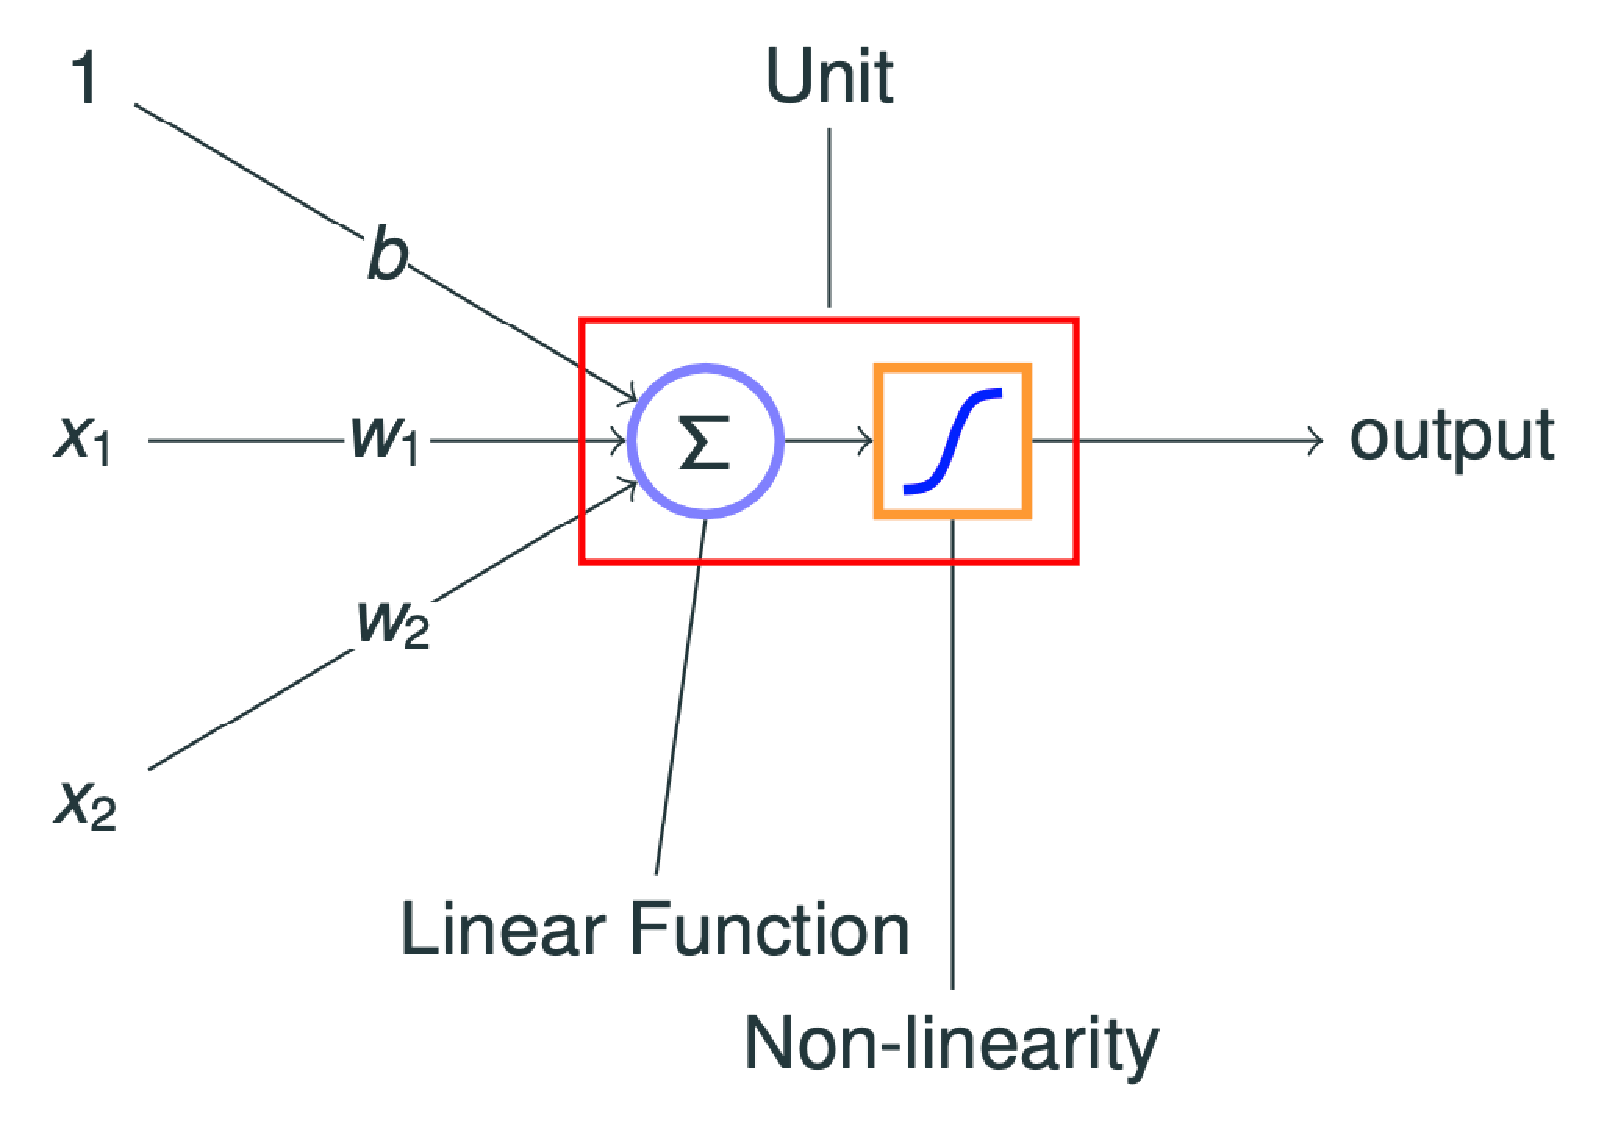
\includegraphics[width = 0.5\textwidth]{simplenn.pdf}
    \end{center}
\end{figure}


Multi-layer neural networks consist of input and output layers and multiple hidden layers. The idea behind using hidden layers is that layers should perform feature extraction.

We consider multi-layer perceptrons which consist of fully connected, feedforward layers. Notation:
\begin{itemize}
	\item $w_{i j}^{\ell}$ : weight for the connection to unit $i$ in layer $\ell$ from unit $j$ in layer $\ell-1$
	\item $b_i^{\ell}:$ bias term for unit $i$ in layer $\ell$
	\item $z_i^{\ell}$ : pre-activation for unit $i$ in layer $\ell$, sum of weighted outputs from $\ell-1$
	\item $a_i^{\ell}$ : activation for unit $i$ in layer $\ell$, non-linear function of pre-activation.\footnote{Note: one activation function per unit, thus $\mathbf{a}^\ell$ is a column vector.}
	\item Weights, etc. in matrix form: each \emph{row} corresponds to one unit. E.g.,
	\begin{equation*}
		\mathbf{W}^k =
		\begin{pmatrix}
			w_{11}^k & w_{12}^k \\
			w_{21}^k & w_{22}^k
		\end{pmatrix}
	\end{equation*}
	the first row corresponds to all weights for unit 1 in layer $k$.
	\item View derivatives as row vectors,
	\begin{equation*}
		\frac{\partial f}{\partial \mathbf{z}}=\left[\begin{array}{lll}
			\frac{\partial f}{\partial z_1} & \cdots & \frac{\partial f}{\partial z_n}
			\end{array}\right]
	\end{equation*}
	\item Derivative of multi-variate function with respect to vector, example:
	\begin{equation*}
		\frac{\partial \mathbf{a}^2}{\partial \mathbf{z}^2}=\left[\begin{array}{ll}
			\frac{\partial a_1^2}{\partial z_1^2} & \frac{\partial a_1^2}{\partial z_2^2} \\
			\frac{\partial a_2^2}{\partial z_1^2} & \frac{\partial a_2^2}{\partial z_2^2}
			\end{array}\right]
	\end{equation*}

\end{itemize}

\subsection{Model Learning}

Idea:
\begin{itemize}
	\item Compute derivatives for all parameters for each data point
	\item Average derivatives
	\item Perform gradient descent step to update parameters
	\begin{itemize}
		\item Error propagated back to every layer
		\item Weights in matrix adjust proportional to error and weights
	\end{itemize}
\end{itemize}

Backpropagation excessively uses the chain rule to compute derivatives in modular and efficient fashion, by reusing deriatives to ease computation.

\subsubsection*{Chain Rule:}

Functions $f: \mathbb{R}^n \rightarrow \mathbb{R}^k, g: \mathbb{R}^k \rightarrow \mathbb{R}^m, h=g \circ f: \mathbb{R}^n \rightarrow \mathbb{R}^m$.


For $\mathbf{x} \in \mathbb{R}^n$, let $\mathbf{z}=f(\mathbf{x}), h =g({f(x)})$
$$
\frac{\partial h}{\partial \mathbf{x}}=  \frac{\partial h}{\partial \mathbf{z}} \frac{\partial \mathbf{z}}{\partial \mathbf{x}}
$$
\begin{itemize}
	\item $\frac{\partial h}{\partial \mathbf{x}}$ is an $m \times n$ Jacobian matrix
	\item $\frac{\partial h}{\partial z}$ is an $m \times k$ Jacobian matrix
	\item $\frac{\partial \mathbf{z}}{\partial \mathbf{x}}$ is an $k \times n$ Jacobian matrix
\end{itemize}

\subsubsection*{Backpropagation Algorithm}

Assume all layers are fully connected. Layer $I$  consists of the following:
$$
\begin{aligned}
& \mathbf{z}^{\prime}=\mathbf{W}^{\prime} \mathbf{a}^{\prime-1}+\mathbf{b}^{\prime} \\
& \mathbf{a}^{\prime}=f_l\left(\mathbf{z}^{\prime}\right)
\end{aligned}
$$
where $f_l$ is the non-linear activation in layer $I$.

If there are $n_l$ units in layer $I$, then $\mathbf{W}^{I} \in \mathbb{R}^{n_l \times n_{l-1}}$.

\noindent\emph{Forward pass:}

\begin{enumerate}
	\item $\mathbf{a}^1=\mathbf{x} \text { (input) }$
	\item $\mathbf{z}^{\prime}=\mathbf{W}^{\prime} \mathbf{a}^{I-1}+\mathbf{b}^{\prime}$
	\item $\mathbf{a}^{\prime}=f_l\left(\mathbf{z}^{\prime}\right)$  (May map vector- or elementwise)
	\item $\ell\left(\mathbf{a}^L, y\right)$
\end{enumerate}

\noindent\emph{Backward pass}

Consider the last layer $L$:

\begin{equation*}
	\begin{aligned}
		& \mathbf{z}^L=\mathbf{W}^L \mathbf{a}^{L-1}+\mathbf{b}^L \\
		& \mathbf{a}^L=f_L\left(\mathbf{z}^L\right) \\
		& \text { Loss: } \quad \ell\left(y, \mathbf{a}^L\right) \\
		& \frac{\partial \ell}{\partial \mathbf{z}^L}=\frac{\partial \ell}{\partial \mathbf{a}^L} \frac{\partial \mathbf{a}^L}{\partial \mathbf{z}^L}
		\end{aligned}
\end{equation*}

Arbitrary layer $I$:

We have:
\begin{itemize}
	\item Inputs into layer $I+1$, $\mathbf{a}^I$
	\item $\mathbf{z}^{\prime+1}=\mathbf{W}^{\prime+1} \mathbf{a}^{\prime}+\mathbf{b}^{\prime+1}$ where $w_{j,k}^{I+1}$ weight on connectrion of k-th unit in layer $I$ to $j$-th unit in layer $I+1$
	\item Activation function, $\mathbf{a}^{\prime}=f\left(\mathbf{z}^{\prime}\right)$
	\item Derivative passed from previous layer, $\frac{\partial \ell}{\partial z^{I+1}}$
\end{itemize}

We can then compute:

\begin{equation*}
	\begin{aligned}
		\frac{\partial \ell}{\partial \mathbf{z}^{I}} & =\frac{\partial \ell}{\partial \mathbf{z}^{I+1}} \frac{\partial \mathbf{z}^{I+1}}{\partial \mathbf{z}^{I}} \\
		& =\frac{\partial \ell}{\partial \mathbf{z}^{I+1}} \frac{\partial \mathbf{z}^{I+1}}{\partial \mathbf{a}^{I}} \frac{\partial \mathbf{a}^{I}}{\partial \mathbf{z}^{I}} \\
		& =\frac{\partial \ell}{\partial \mathbf{z}^{I+1}} \mathbf{W}^{I+1} \frac{\partial \mathbf{a}^{I}}{\partial \mathbf{z}^{I}}
	\end{aligned}
\end{equation*}

We obtain the derivatives wrt $w_{i j}^{I}$ and $b_i^{I}$ using $\frac{\partial \ell}{\partial z^{I}}$ :
\begin{itemize}
	\item $\frac{\partial \ell}{\partial w_{i j}^I}=\frac{\partial \ell}{\partial z_i^{I}} \frac{\partial z_j^I}{\partial w_{i j}^I}=\frac{\partial \ell}{\partial z_i^I} a_j^{I-1}$ or $\frac{\partial \ell}{\partial \mathbf{W}^{I}}=\left(a^{I-1} \frac{\partial \ell}{\partial \mathbf{z}^{I}}\right)^{\top}$
	\item $\frac{\partial \ell}{\partial b_i^{I}}=\frac{\partial \ell}{\partial z_i^{I}}$ or $\frac{\partial \ell}{\partial \mathbf{b}^{I}}=\frac{\partial \ell}{\partial \mathbf{z}^{I}}$
\end{itemize}

Takeaway: Instead of computing each derivative separately, we only need to compute $\frac{\partial \ell}{\partial \mathbf{z}^{I}}$ and use the chain rule.

\subsubsection*{Computational requirements}

\begin{itemize}
	\item As many matrix multiplications as fully connected layers
	\item Performed twice during forward nacd backward pass
	\item Must store $\mathbf{a}^{I}, \mathbf{z}^{I} \text {, and } \frac{\partial \ell}{\partial \mathbf{z}^{I}}$ for each layer
\end{itemize}


\subsection{Challenges in training deep NNs}

Main challenges:
\begin{itemize}
	\item Backpropagation is computationally expensive, instead use mini-batch SGD
	\item Overfitting
	\item May not converge
\end{itemize}


\emph{Saturation issue}: Activation function may be in very flat region, thus gradients are very small. Using different loss functions may partially aleviate the issue.\footnote{E.g., using a cross-entropy loss function leads to some cancelling out of activation gradients which can be useful.}

\emph{Vanishing gradient problem}: Products of many gradients which are small can often be $\approx 0$. In backpropagation, one also multiplies with weights, this can explode the gradient instead.

Can avoid saturation using ReLU: $f(z)=\max (0, z)$.
\begin{itemize}
	\item Only saturates one side as derivative is constant for large $z$ (thus avoids saturation)
	\item Sparsely activated, some neurons may not activate at all
	\item Dying ReLU problem: once deactivated, unlikely to reactivate
	\begin{itemize}
		\item Can use leaky (parametric) ReLU instead, but can no longer have sparse activation:
		\begin{equation*}
			f(z)= \begin{cases}a z & \text { if } z<0 \\ z & \text { if } z \geq 0\end{cases}
		\end{equation*}
	\end{itemize}
\end{itemize}


\emph{Initialising weights}: Due to non-convexity, we only find local optima. Initial weights are therefore important for convergence and solution.

\begin{itemize}
	\item Weight initialisation for sigmoid/ReLU units
	\begin{itemize}
		\item Suppose there are $D$ weights $w_1, \ldots, w_D$
		\item Draw $w_i$ randomly from $\mathcal{N}\left(0, \frac{1}{D}\right)$
	\end{itemize}
	\item Bias initialisation:
	\begin{itemize}
		\item For sigmoid: Use a random value around 0
		\item For ReLU: Use a small positive constant
	\end{itemize}
\end{itemize}


\emph{Overfitting}:
\begin{itemize}
	\item Early stopping:
	\begin{itemize}
		\item Measure performance on validation set after each gradient step
		\item Stop when validation error stops decreasing
	\end{itemize}
	\item Modified data:
	\begin{itemize}
		\item Create fake data by changing brightness, etc.
		\item Adversarial training: take trained model and create examples by adding noise impercetbily to human eye such that model makes errors.
	\end{itemize}
	\item Bagging:
	\begin{itemize}
		\item General idea, train models on different samples obtained by sampling with replacement.
		\item In NN: \emph{Dropout}.
		\item Ignore fraction of hidden units in each traning step
		\item Prevents co-adoption among different neurons
		\item At test time, use complete model
		\item Must re-scale weights. E.g., if dropout rate was 1/2, halve all weights
	\end{itemize}
\end{itemize}

\section{Clustering}

Idea: Unsupervised learning problem. Group together data into subsets such that dissimilarity between items within a group is minimized.

Two types of algorithms:
\begin{enumerate}
	\item Feature based: points are vectors in $\mathbb{R}^D$
	\item Dis-similarity based: data consists of pairwise dissimilarities of data points
\end{enumerate}

\subsubsection*{K-Means Clustering}

Partition data into subsets $C_1, ..., C_k$ with fixed $k$. Measure quality of partition:
\begin{equation*}
	W(C)=\frac{1}{2} \sum_{j=1}^k \frac{1}{\left|C_j\right|} \sum_{i, i^{\prime} \in C_i} d\left(\mathbf{x}_i, \mathbf{x}_{i^{\prime}}\right)
\end{equation*}
With euclidian distance, this simplifies to $W(C)=\sum_{j=1}^k \sum_{i \in \mathcal{C}_j}\left\|\mathbf{x}_i-\boldsymbol{\mu}_j\right\|_2^2$ where $\boldsymbol{\mu}_j=\frac{1}{\left|C_j\right|} \sum_{i \in C_j} \mathbf{x}_i$.

Objective: minimise the sum of squares of distances to the mean within each cluster.
\begin{itemize}
	\item Joint minimization over partitions and means is np-hard due to combinatorial nature of problem.
	\item Instead use \textbf{Lloyd's Algorithm}: After initialising means randomly, repeat until convergence (means to do not change).
	\begin{enumerate}
		\item Construct clusters $C_1, \ldots, C_k$ by assigning the data to clusters represented by their means:
		$$
		C_j=\left\{i \mid j=\underset{j^{\prime}}{\operatorname{argmin}}\left\|\mathbf{x}_i-\boldsymbol{\mu}_{j^{\prime}}\right\|_2^2\right\}
		$$
		\item Update means using the current cluster assignments:
		$$
		\boldsymbol{\mu}_j=\frac{1}{\left|C_j\right|} \sum_{i \in C_j} \mathbf{x}_i
		$$
	\end{enumerate}
	\item Algorithm always converges to a \emph{local} minimum as only finitely many partitions.\footnote{At each iteration, means only change if a point changed clusters, in which case the mean updating will automatically lead to a lower value of the target function (as the mean minmizes the function $\sum_i (x_i- \mu)^2$). Thus value function always decreases until convergence. After each possible assignment was seen once it cannot be that the objective function still decreases, thus the algorithm must converge in $k^N$ iterations.}
	\item $k$ hyperparamter, chosen based on kink in test MSE
	\item Extensions:
	\begin{itemize}
		\item k-medoids: use data points as cluster means, use any distance not necessarily euclidian.
		\item k-center: Objective: maximum over all dissimilarities between data and anchor
	\end{itemize}
	\item Note: Decision boundary will be linear. Same distance from two centers so $||\mathbf{x}- \mu_1||^2 = ||\mathbf{x}- \mu_2||^2$. Expaning and simplyfing leads to
	\begin{equation*}
		\left(\mu_1 - \mu_2\right) \mathbf{x}  + \left(||\mu_1||^2-||\mu_2||^2\right) / 2 = 0
	\end{equation*}
	which is a hyperplane.
\end{itemize}

\subsubsection*{Transforming between dissimilarities and numeric features}

\noindent\emph{From $\mathbb{R}^D$ to dissimilarities:}

Given feature vectors, we can obtain dissimilarities by applying
\begin{equation*}
	d\left(\mathbf{x}, \mathbf{x}^{\prime}\right)=f\left(\sum_{i=1}^D w_i d_i\left(x_i, x_i^{\prime}\right)\right).
\end{equation*}


\noindent\emph{From dissimilarities to $\mathbb{R}^D$:}

Assume $D_{i j}=\left\|\mathbf{x}_i-\mathbf{x}_j\right\|_2^2, \text { for } i, j \in[N]$ is given, we want to find $\mathbf{x}_i$ for $i =1, \dots, N$. I.e., we have dissimilarities and want to recover points in the euclidian space from this dissimilarity matrix.\footnote{As we require points in the euclidian space to apply k-means.} Finding a Euclidian embedding of data that approximately respects original dissimilarities is called \textbf{multidimensional scaling.}

\begin{itemize}
	\item Given assumption of euclidian distance, we have
	\begin{align*}
		D_{i j} & =\left\|\mathbf{x}_i-\mathbf{x}_j\right\|_2^2 \\
		& =\mathbf{x}_i^{\top} \mathbf{x}_i-2 \mathbf{x}_i^{\top} \mathbf{x}_j+\mathbf{x}_j^{\top} \mathbf{x}_j \\
		& =M_{i j}-2 M_{i j}+M_{i j}
	\end{align*}
	where $\mathbf{M}=\mathbf{X} \mathbf{X}^{\top} \text { is the } N \times N$ matrix of dot products: $M_{i j}=\mathbf{x}_i \cdot \mathbf{x}_j$
	\item $\mathbf{M}$ can be recovered from $\mathbf{D}$ up to translation.
	\item Obtain $\tilde{\mathbf{x}}_1, \ldots, \tilde{\mathbf{x}}_N \text { from } \mathbf{M}$ using SVD: For $\mathbf{X} \in \mathbb{R}^{N \times D}$, the SVD is $\mathbf{X}=\mathbf{U} \boldsymbol{\Sigma} \mathbf{V}^{\top}$ where
	\begin{itemize}
		\item $\mathbf{U} \in \mathbb{R}^{N \times D}$ and $\mathbf{V} \in \mathbb{R}^{D \times D}$ are orthonormal matrices
		\item $\boldsymbol{\Sigma} \in \mathbb{R}^{D \times D}$ is diagonal with $\sigma_1 \geq \sigma_2 \geq \cdots \geq \sigma_D \geq 0$
		\item $\mathbf{U}^{\top} \mathbf{U}=\mathbf{V}^{\top} \mathbf{V}=\mathbf{I}_D$
	\end{itemize}
	\item  For square, symmetirc, psd matrix $\mathbf{M}$, we can obtain Eigendecomposition: $\mathbf{V}=\mathbf{U}: \mathbf{M}=\mathbf{U} \Sigma \mathbf{U}^{\top}$
	\begin{enumerate}
		\item Let $\tilde{\mathbf{X}}=\mathbf{U} \boldsymbol{\Sigma}^{1 / 2}$
		\item Then
		$$
		\tilde{\mathbf{X}} \tilde{\mathbf{X}}^{\top}=\mathbf{U} \boldsymbol{\Sigma}^{1 / 2}\left(\mathbf{U} \boldsymbol{\Sigma}^{1 / 2}\right)^{\top}=\mathbf{U} \boldsymbol{\Sigma}^{1 / 2} \boldsymbol{\Sigma}^{1 / 2} \mathbf{U}^{\top}=\mathbf{U} \boldsymbol{\Sigma} \mathbf{U}^{\top}=\mathbf{M}
		$$
		\item We recover $\tilde{\mathbf{x}}_i$ as rows of $\mathbf{U} \boldsymbol{\Sigma}^{1 / 2}$.
	\end{enumerate}
\end{itemize}

More generally, we use a mercer kernel to define the similarity between points, thus $\mathbf{M}$ is symmetric and psd, we can find points $\tilde{\mathbf{x}}_i$ using above derivation.

We can view this problem as a non-convex optimization problem,
\begin{equation*}
	\underset{\tilde{\mathbf{x}}_1, \ldots, \tilde{\mathbf{x}}_N}{\operatorname{argmin}} \sum_{i \neq j}\left(\left\|\tilde{\mathbf{x}}_i-\tilde{\mathbf{x}}_j\right\|_2^2-D_{i j}\right)^2
\end{equation*}
which gives us the degree to which we can represent $\mathbf{D}$ in Euclidian space.

\subsubsection*{Hierarchical Clustering}

Idea: build larger clusters and smaller clusters within. Two approaches:
\begin{enumerate}
	\item Agglomerative: bottom-up, merge smaller clusters
	\item Divisie: top-down, split larger clusters
\end{enumerate}
Can be visualized in a \emph{dendrogram}. Cutting this binary tree at a certain levels gives a data partition.


Suppose we have dissimilarity at datapoint level, e.g., $d\left(\mathbf{x}, \mathbf{x}^{\prime}\right)=\left\|\mathbf{x}-\mathbf{x}^{\prime}\right\|$.\footnote{Note: we can therefore apply hierarchical clustering if we only have dissimilarities, we do not require points in Euclidian space.} Define dissimilarity at cluster level, say $C$ and $C^{\prime}$
\begin{itemize}
	\item Single Linkage
	$$
	D\left(C, C^{\prime}\right)=\min _{\mathbf{x} \in C, \mathbf{x}^{\prime} \in C^{\prime}} d\left(\mathbf{x}, \mathbf{x}^{\prime}\right)
	$$
	\item Complete Linkage
	$$
	D\left(C, C^{\prime}\right)=\max _{\mathbf{x} \in C, \mathbf{x}^{\prime} \in C^{\prime}} d\left(\mathbf{x}, \mathbf{x}^{\prime}\right)
	$$
	\item Average Linkage
	$$
	D\left(C, C^{\prime}\right)=\frac{1}{|C| \cdot\left|C^{\prime}\right|} \sum_{\mathbf{x} \in C, \mathbf{x}^{\prime} \in C^{\prime}} d\left(\mathbf{x}, \mathbf{x}^{\prime}\right)
	$$
\end{itemize}

Linkage-based clustering algorithm:
\begin{enumerate}
	\item Initialise clusters as singletons $C_i=\{i\}$
	\item Initialise clusters available for merging $S=\{1, \ldots, N\}$
	\item Repeat
	\begin{enumerate}
		\item Pick 2 most similar clusters, $(j, k)=\underset{j, k \in S}{\operatorname{arg min }} \; D(j, k)$
		\item Let $C_I=C_j \cup C_k$ for some new index $I$
		\item If $C_I=\{1, \ldots, N\}$, break;
		\item Update $S:=(S \backslash\{j, k\}) \cup\{I\}$
		\item Update $D(i, I)$ for all $i \in S$ (using desired linkage property)
	\end{enumerate}
\end{enumerate}

\subsubsection*{Spectral Clustering}

Method for finding non-convex clusters.

Approach:

\begin{enumerate}
	\item Construct $K$-nearest neighbour graph from data
	\begin{itemize}
		\item One node for every point in dataset
		\item $(i, j)$ is an edge if either $i$ is among the $K$ nearest neighbours of $j$ or vice versa
		\item The weight of edge $(i, j)$, if exists,  given by similarity measure $s_{i, j}$
		$$
		s_{i, j}=\exp \left(-\left\|\mathbf{x}_i-\mathbf{x}_j\right\|^2 / \sigma\right)
		$$
	\end{itemize}
	\item Use graph partitioning algorithms, e.g., Laplacian:\footnote{We want to find cuts such that the cut cost is minimized. I.e., weights of edges between two points at boundary should be small. Mincuts with only one node on each side of the cut can often give bad cuts, multi-way cuts are NP-hard. Instead we relax the problem.}
	\begin{enumerate}
		\item $\mathbf{W}$ is the weighted adjacency matrix, $\mathbf{D }$ is (diagonal) degree matrix $D_{i i}=\sum_j W_{i j}$, Laplacian $\mathbf{L}=\mathbf{D}-\mathbf{W}$
		\item Calculate eigenvectors of $\mathbf{L}$
		\item Use matrix of eigenvectors $[\mathbf{v}_2 \dots \mathbf{v}_d]$ as $N \times (d-1)$ feature matrix\footnote{Note that vector of one's is always an eigenvector due to structure of $\mathbf{L}$. We are interested in the eigenvectors corresponding to the smallest eigenvalues.}
		\item Apply K-means to this representation
	\end{enumerate}
\end{enumerate}

The usefulness of the Laplacian comes from the idea of minimizing cut costs while relaxing some constraints. Originally, goal would be to find value binary values $x = \pm 1$ such that each point, depending on the cluster to which the point is assinged equals $1$ or $-1$. We do this to optimize the edge weight objective function given by $\sum_{i, j} w_{i j}\left(x_i-x_j\right)^2$. We relax this, and allow for real-valued $x$, while requiring $\sum_i x_i = 0$ (balanced partition) and $x^Tx = 1$ (normalisation).

We have
\begin{equation*}
	\begin{aligned}
		x^{\top} \mathbf{L} x&=x^{\top}(\mathbf{D}-\mathbf{W}) x \\
		&= \sum_i \sum_j w_{i j}\left(\frac{1}{2} x_i^2+\frac{1}{2} x_j^2\right)-\sum_i \sum_j w_{i j} x_i x_j \\
		&= \sum_i \sum_j w_{i j}\left(x_i-x_j\right)^2 / 2
	\end{aligned}
\end{equation*}
Thus, minimizing $x^T \mathbf{L} x$ is closely related to minimizing cut cost. Since $x^Tx = 1$, we have
\begin{equation*}
	\min x^T \mathbf{L} x = \min \frac{x^T \mathbf{L} x}{x^T x}
\end{equation*}
This is the \emph{Rayleigh quotient} which is minimized when choosing $x$ to be an eigenvector of $\mathbf{L}$.



\section{PCA}

Real-life data may be redundant (e.g., correlation among features). Goal \textbf{Dimensionality Reduction}: Obtain a lower dimensional representation of data while minimizing information loss.

PCA in a nutshell:

\begin{enumerate}
	\item Standardize input data $\mathbf{X} \in \mathbb{R}^{N \times D}$
	\item Compute covariance matrix $\mathbf{X}^T \mathbf{X}$ to identify correlations
	\item  Compute eigenvectors of $\mathbf{X}^T \mathbf{X}$ to identify principal components. $k$-th PC is eigenvector corresponding to $k$-th largest eigenvalue
\end{enumerate}

The idea is that eigenvectors represent the directions of the data that explain the largest variance in the data and thus also minimize information loss. Two equivalent views:
\begin{enumerate}
	\item Maximum variance: find $k$ directions to maximize variance in data
	\item Best reconstruction: find $k$ dimensional subspace with smallest reconstruction error
\end{enumerate}

\subsubsection*{Maximum variance view}

\begin{itemize}
	\item Given: Dataset $\mathbf{X} \in \mathbb{R}^{N \times D}$ with $N$ data points of $D$ dimensions as row vectors
	\item Goal: Find unit vector $\mathbf{v}_1 \in \mathbb{R}^D$ that maximises the variance of the dataset of the projections $\mathbf{x}_i \cdot \mathbf{v}_1$ of the data points $\mathbf{x}_i$ onto $\mathbf{v}_1$
	\item Solution:
	\begin{align}
		\mathbf{v}_1&=\underset{\mathbf{v}_1:\left\|\mathbf{v}_1\right\|=1}{\operatorname{argmax}}\left(\sum_{i \in[N]}\left(\mathbf{x}_i \cdot \mathbf{v}_1\right)^2\right)=\underset{\mathbf{v}_1:\left\|\mathbf{v}_1\right\|=1}{\operatorname{argmax}}\left(\left\|\mathbf{X} \mathbf{v}_1\right\|^2\right) \notag \\
		&=\underset{\mathbf{v}_1:\left\|\mathbf{v}_1\right\|=1}{\operatorname{argmax}}\left(\mathbf{v}_1^{\top} \mathbf{X}^{\top} \mathbf{X}_1 \mathbf{v}_1\right) \label{eq.pcamaxvar}
	\end{align}
	\item Next find $\mathbf{v}_2, \mathbf{v}_3, \ldots, \mathbf{v}_k$ that are all successively orthogonal to previous directions and maximise (as yet unexplained) variance\footnote{Note that
	\begin{equation*}
		\begin{aligned}
			\widehat{\mathbf{X}}_j \mathbf{v}_j & =\mathbf{X} \mathbf{v}_j-\mathbf{X} \mathbf{v}_1 \mathbf{v}_1^{\top} \mathbf{v}_j-\cdots-\mathbf{X} \mathbf{v}_{j-1} \mathbf{v}_{j-1}^{\top} \mathbf{v}_j \\
			& =\mathbf{X} \mathbf{v}_j \text { (due to orthogonality) }
		\end{aligned}
	\end{equation*}
	so we obtain $\mathbf{v}_j =\underset{\mathbf{v}_j:\left\|\mathbf{v}_j\right\|=1, \mathbf{v}_j \perp \mathbf{v}_1, \ldots, \mathbf{v}_j \perp \mathbf{v}_{j-1}}{\operatorname{argmax}}\left(\mathbf{v}_j^{\top} \mathbf{X}^{\top} \mathbf{X} \mathbf{v}_j\right)$.
	}
	$$
	\widehat{\mathbf{X}}_j=\mathbf{X}-\sum_{s=1}^{j-1} \mathbf{X v}_s \mathbf{v}_s^{\top}, \quad 1 \leq j \leq k
	$$
\end{itemize}

Note that the solution for \eqref{eq.pcamaxvar} again follows from Rayleigh's quotient. The optimal vector is the eigenvector corresponding to the largest eigenvalue of $\mathbf{X}^\top \mathbf{X}$.


\subsubsection*{Reconstruction view}

\begin{itemize}
	\item Given: Dataset $\mathbf{X} \in \mathbb{R}^{N \times D}$ with $N$ rows vectors $\mathbf{x}_1, \ldots, \mathbf{x}_N$
	\item Goal: Find a $k$-dimensional linear projection that best represents the data
	Solution in case of one PC:
	\begin{enumerate}
		\item Let $\mathbf{v}_1$ be the direction of projection
		\item The point $\mathbf{x}_i$ is mapped to $\tilde{\mathbf{x}}_i=\left(\mathbf{v}_1 \cdot \mathbf{x}_i\right) \mathbf{v}_1$, where $\left\|\mathbf{v}_1\right\|=1$\footnote{Recall: The vector projection of a vector $\mathbf{v}$ on a nonzero vector $\mathbf{u}$ is defined as $\operatorname{proj}_{\mathbf{u}}(\mathbf{v})=\frac{\langle\mathbf{v}, \mathbf{u}\rangle}{\langle\mathbf{u}, \mathbf{u}\rangle} \mathbf{u}$. Thus, $\tilde{\mathbf{x}}_i$ is the projection of $\mathbf{x}_i$ onto the vector $\mathbf{v}_1$.}
		\item Minimise reconstruction error $\sum_{i=1}^N\left\|\mathbf{x}_i-\tilde{\mathbf{x}}_i\right\|^2$
	\end{enumerate}
	\item Solution in case of $k$ PCs:
	\begin{itemize}
		\item Suppose $\mathbf{V}_k \in \mathbb{R}^{D \times k}$ is such that columns of $\mathbf{V}_k$ are orthogonal
		\item Project data $\mathbf{X}$ onto subspace defined by $\mathbf{V}_k: \mathbf{Z}=\mathbf{X} \mathbf{V}_k$ are coordinates of our data in the lower-dimensional space
		\item Mapping back to the original space, $\tilde{\mathbf{X}} = \mathbf{X} \mathbf{V}_k \mathbf{V}_k^\top$\footnote{Note that this follows from the usual form of the projection matrix since $\mathbf{V}_k$ is orthonormal. I.e., $\mathbf{P}_\mathbf{X} =  \mathbf{X}(\mathbf{X}^\top \mathbf{X})^{-1}\mathbf{X}^\top$ which reduces to $\mathbf{X}\mathbf{X}^\top$.}
		\item Minimise reconstruction error $\sum_{i=1}^N\left\|\mathbf{x}_i-\mathbf{V}_k \mathbf{V}_k^{\top} \mathbf{x}_i\right\|^2$
	\end{itemize}
\end{itemize}

\subsubsection*{Equivalence}

\begin{itemize}
	\item Maximum Variance: Find $\mathbf{v}_1$ that maximises $\sum_{i=1}^N\left(\mathbf{v}_1 \cdot \mathbf{x}_i\right)^2$
	\item Best Reconstruction: Find $\mathbf{v}_1$ that minimises:
	$$
	\begin{aligned}
	\sum_{i=1}^N\left\|\mathbf{x}_i-\tilde{\mathbf{x}}_i\right\|^2 & =\sum_{i=1}^N\left(\left\|\mathbf{x}_i\right\|^2-2\left(\mathbf{x}_i \cdot \tilde{\mathbf{x}}_i\right)+\left\|\tilde{\mathbf{x}}_i\right\|^2\right) \\
	& =\sum_{i=1}^N\left(\left\|\mathbf{x}_i\right\|^2-2\left(\mathbf{v}_1 \cdot \mathbf{x}_i\right)^2+\left(\mathbf{v}_1 \cdot \mathbf{x}_i\right)^2\left\|\mathbf{v}_1\right\|^2\right) \\
	& =\sum_{i=1}^N\left\|\mathbf{x}_i\right\|^2-\sum_{i=1}^N\left(\mathbf{v}_1 \cdot \mathbf{x}_i\right)^2
	\end{aligned}
	$$
\end{itemize}

\subsubsection*{PCA and SVD}

The maximum variance view shows us that we can obtain our principal components from the eigenvectors of $\mathbf{X}^\top \mathbf{X}$. From the reconstruction point, we have a useful theoretical result which we can use:

\begin{theorem}[Eckart-Young]
	Let $\mathbf{X}$ be a real $N \times D$ matrix and denote by $\mathbf{X}_k$ the singular value decomposition of $\mathbf{X}$ truncated at rank $k$. Then for any $k \in \mathcal{N}$ and any $N \times D$ matrix $\mathbf{Y}$ of rank at most $k$, we have $\left\|\mathbf{X}-\mathbf{X}_k\right\|_F \leq\|\mathbf{X}-\mathbf{Y}\|_F$.\footnote{The Frobenius norm of the matrix $\mathbf{X} \in \mathbb{R}^{N \times D}$, denoted $\|\mathbf{X}\|_F$, is defined by
	 $$
	 \|\mathbf{X}\|_F=\sqrt{\sum_{i=1}^N \sum_{j=1}^D x_{i j}^2}=\sqrt{\operatorname{tr}\left(\mathbf{X}^{\top} \mathbf{X}\right)}
	 $$
	 }
\end{theorem}

I.e., we can find our optimal reconstruction by considering the truncated singular value decomposition of $\mathbf{X}$.

Since $\mathbf{X}=\mathbf{U} \boldsymbol{\Sigma} \mathbf{V}^{\boldsymbol{\top}}$, we obtain
\begin{equation*}
	\mathbf{X}^{\top} \mathbf{X}=\left(\mathbf{U} \boldsymbol{\Sigma} \mathbf{V}^{\top}\right)^{\boldsymbol{\top}}\left(\mathbf{U} \boldsymbol{\Sigma} \mathbf{V}^{\top}\right)= \mathbf{V}  \boldsymbol{\Sigma}^{\boldsymbol{\top}} \boldsymbol{\Sigma}  \mathbf{V}^{\boldsymbol{\top}}
\end{equation*}
Eivdently, this is the eigendecomposition of the psd matrix $\mathbf{X}^\top \mathbf{X}$. Thus,
\begin{itemize}
	\item the eigenvectors of $\mathbf{X}^{\top} \mathbf{X}$ are the right singular vectors $\mathbf{v}_i$ of $\mathbf{X}$
	\item the eigenvalues of $\mathbf{X}^{\top} \mathbf{X}$ are the squares of the singular values $\sigma_i$ of $\mathbf{X}$
	\item Similarly, the eigenvectors $\mathbf{u}_j$ of $\mathbf{X X}^{\top}$ with eigenvalue $\sigma^2$ are the left singular vectors of $\mathbf{X}$
\end{itemize}

Similar to above, we want to have $\mathbf{Z} = \mathbf{X V}$. Plugging in the SVD and truncating, as we only use $k$ eigenvectors corresponding to largest eigenvalues,  we get:\footnote{$\mathbf{U}_k$ is $N \times k$, $\mathbf{\Sigma}_k$ is $k \times k$, $\mathbf{V}_k^\top$ is $k \times D$ so we end up with $\mathbf{Z}_k \mathbf{V}_k^\top$ again being $N \times D$.}
\begin{equation*}
	\begin{aligned}
		&\mathbf{Z}=\mathbf{X V}=\mathbf{U} \mathbf{\Sigma} \mathbf{V}^{\top} \mathbf{V}=\mathbf{U} \mathbf{\Sigma} \\
		&\mathbf{Z}_k=\mathbf{U}_k \boldsymbol{\Sigma}_k=\mathbf{X} \mathbf{V}_k
	\end{aligned}
\end{equation*}
Note that this also shows that principal components are a linear combination of the original features. (Further, this is an orthonormal linear combination.)

Our reconstruction is then $\tilde{\mathbf{X}} = \mathbf{Z}_k \mathbf{V}_k^\top = \mathbf{X} \mathbf{V}_k \mathbf{V}_k^\top = \mathbf{U}_k \mathbf{\Sigma}_k \mathbf{V}_k^\top$ which is precisely the rank-$k$ truncated SVD of $\mathbf{X}$.


\begin{itemize}
	\item Eckart-Young Theorem shows that minimum reconstruction error is obtained by using the truncated SVD $\mathbf{\tilde{X}} = \mathbf{Z}_k \mathbf{V}_k^T =\mathbf{U}_k \boldsymbol{\Sigma}_k \mathbf{V}_k^{\top}$
	\item Comparison to eigendecomposition: $\mathbf{V}_k$ contains the k eigenvectors of $\mathbf{X}^\top \mathbf{X}$ corresponding to largest eigenvalues
	\item Columns of $\mathbf{V}_k$ are the principal components of $\mathbf{X}$
	\item Columns of $\mathbf{Z}_k$ are the coefficients used to approximate each data point as a linear combination of the principal components
\end{itemize}


\subsubsection*{Algorithms for PCA Constructions}

Suppose $N \gg D$: Either,

\begin{enumerate}
	\item Variant 1: Construct $\mathbf{X}^{\top} \mathbf{X}$ in $O\left(D^2 N\right)$ and its eigenvectors in $O\left(D^3\right)$
	\item Variant 2: Iterative methods to get top $k$ singular (right) vectors directly:
	\begin{enumerate}
		\item Initiate $\mathbf{v}^0$ to be random unit norm vector
		\item Iterative Update:
		\item $\mathbf{v}^{t+1}=\mathbf{X}^{\top} \mathbf{X} \mathbf{v}^t$
		\item $\mathbf{v}^{t+1}=\mathbf{v}^{t+1} /\left\|\mathbf{v}^{t+1}\right\|$
		until (approximate) convergence
		\item Update step takes $O(N D)$ time\footnote{Compute $\mathbf{X} \mathbf{v}^t$ first, then $\mathbf{X}^{\top}\left(\mathbf{X}^t\right)$)}
		\item This gives the singular vector corresponding to the largest singular value. Subsequent singular vectors obtained by choosing $\mathbf{v}^0$ orthogonal to previously identified singular vectors
	\end{enumerate}
\end{enumerate}

$D \gg N$:

\begin{itemize}
	\item Construct $\mathbf{X X}^{\top}$ in $O\left(N^2 D\right)$; eigenvectors of $\mathbf{X} \mathbf{X}^{\top}$ in $O\left(N^3\right)$
	\item The eigenvectors give the left singular vectors, $\mathbf{u}_i$ of $\mathbf{X}$
	\item To obtain $\mathbf{v}_i$, we use $\mathbf{v}_i=\sigma^{-1} \mathbf{X}^{\top} \mathbf{u}_i$
\end{itemize}


\subsubsection*{Reconstruction Error}

Suppose we have $\mathbf{Z}=\mathbf{X} \mathbf{V}_k=\mathbf{U}_k \boldsymbol{\Sigma}_k$, we reconstruct $\mathbf{\tilde{X}} = \mathbf{Z} \mathbf{V}_k^T$. The reconstruction error is:\footnote{This follows from
\begin{equation*}
	\begin{aligned}
		\mathbf{X}=\mathbf{U} \boldsymbol{\Sigma} \mathbf{V}^{\top}=\sum_{j=1}^D \sigma_j \mathbf{u}_j \mathbf{v}_j^{\top}; \; \tilde{\mathbf{X}}=\mathbf{U}_k \boldsymbol{\Sigma}_k \mathbf{V}_k^{\top}=\sum_{j=1}^k \sigma_j \mathbf{u}_j \mathbf{v}_j^{\top}; \; \|\mathbf{X}-\tilde{\mathbf{X}}\|_F^2=\sum_{j=k+1}^D \sigma_j^2
	\end{aligned}
\end{equation*}
}
\begin{equation*}
	\sum_{i=1}^N\left\|\mathbf{x}_i-\mathbf{V}_k \mathbf{V}_k^{\top} \mathbf{x}_i\right\|^2=\sum_{j=k+1}^D \sigma_j^2
\end{equation*}

We may identify the number of PCs to keep by identifiyng a `kink' in plotting $k$ vs reconstruction error, or by using a threshold $t$ such that $\frac{\left\|\mathbf{X}-\mathbf{X}_k\right\|_F^2}{\|\mathbf{X}\|_F^2}=\frac{\sigma_{k+1}^2+\cdots+\sigma_D^2}{\sigma_1^2+\cdots+\sigma_D^2} \leq t$.


\clearpage


\appendix

\section{Mathematical Appendix}

\subsubsection*{Calculation and Derivative Rules for Matrices}

\begin{align*}
	\mathbf{A}(\mathbf{B}+\mathbf{C})=\mathbf{A B}+\mathbf{A C} \\
	(\mathbf{A} \mathbf{B})^T = \mathbf{B}^T \mathbf{A}^T \\
	(\mathbf{A} \mathbf{B})^{-1} = \mathbf{B}^{-1} \mathbf{A}^{-1} \\
	\text{Derivatives:} \\
	\nabla_{\mathbf{x}}\left(\mathbf{c}^{\top} \mathbf{x}\right) & =\mathbf{c} \\
	\nabla_{\mathbf{x}}\left(\mathbf{x}^{\top} \mathbf{x}\right) & =2 \mathbf{x} \\
	\nabla_{\mathbf{x}}(\mathbf{A} \mathbf{x}) & =\mathbf{A}^{\top} \\
	\nabla_{\mathbf{x}}\left(\mathbf{x}^{\top} \mathbf{A} \mathbf{x}\right) & =\mathbf{A} \mathbf{x}+\mathbf{A}^{\top} \mathbf{x}
\end{align*}

\subsubsection*{Determinant calculation}

Let $\mathbf{A}$ be an $n \times n$ matrix for some $n \geq 1$. If $\mathbf{A}$ consists of a single element, then the determinant $\operatorname{det}(\mathbf{A})$ of $\mathbf{A}$ is the element itself. Otherwise:
$$
\operatorname{det}(\mathbf{A})=\left|\begin{array}{cccc}
a_{1,1} & a_{1,2} & \cdots & a_{1, n} \\
a_{2,1} & a_{2,2} & \cdots & a_{2, n} \\
\vdots & \vdots & \ddots & \vdots \\
a_{n, 1} & a_{n, 2} & \cdots & a_{n, n}
\end{array}\right|=\sum_{j=1}^n(-1)^{i+j} a_{i, j} M_{i, j},
$$
where $i \in[n]$ is arbitrary and $M_{i, j}$ (called minor) is the determinant of $\mathbf{A}$ after removing the $i$-th row and $j$-th column.

For a $2 \times 2$ matrix:
\begin{equation*}
	\det
	\begin{pmatrix}
		a & b \\
		c & d
	\end{pmatrix}
	= ad - bc
\end{equation*}

\subsubsection*{Inverse calculation}

For a $2 \times 2$ matrix $A$, we have
\begin{equation*}
	A^{-1} =
	\begin{pmatrix}
		a & b \\
		c & d
	\end{pmatrix}^{-1}
	=
	\frac{1}{\det A}
	\begin{pmatrix}
		d & -b \\
		-c & a
	\end{pmatrix}
\end{equation*}





For a 3x3 matrix A, its inverse $A^{-1}$ can be calculated using the formula:

$$
A^{-1} = \frac{1}{\det(A)} \cdot \text{adj}(A)
$$
where $\det(A)$ is the determinant and $\text{adj}(A)$ is the adjugate matrix.

\begin{enumerate}
	\item For each element $a_{ij}$, calculate its cofactor $C_{ij}$ using:
	$$C_{ij} = (-1)^{i+j} \cdot M_{ij}$$
	where $M_{ij}$ is the minor (determinant of the 2x2 matrix formed by deleting row i and column j).
	\item The adjugate matrix is the transpose of the cofactor matrix:
	$$\text{adj}(A) = C^T$$
	\item Multiply the adjugate matrix by the reciprocal of the determinant:
	$$A^{-1} = \frac{1}{\det(A)} \begin{pmatrix} C_{11} & C_{21} & C_{31} \\ C_{12} & C_{22} & C_{32} \\ C_{13} & C_{23} & C_{33} \end{pmatrix}$$
\end{enumerate}







\section{Complexity of matrix computations}


\begin{itemize}
	\item Matrix Inversion ($N \times N$ matrix):
	\begin{itemize}
		\item Complexity: $O(N^3)$
		\item Explanation: $N$ steps of elimination, each with $O(N^2)$ operations
	\end{itemize}
	\item Matrix-Matrix Multiplication: $N \times M$ matrix times $M \times P$ matrix:
	\begin{itemize}
		\item Complexity: $O(N \times M \times P)$
		\item Explanation: $M$ operations for each element of $N \times P$ result
	\end{itemize}
	\item Matrix-Vector Multiplication: $N \times M$ matrix times $M \times 1$ vector:
		\begin{itemize}
			\item Complexity: $O(N \times M)$
			\item Explanation: $M$ operations for each of $N$ output elements
		\end{itemize}
	\item Vector-Vector Multiplication:
	\begin{itemize}
		\item Inner product ($1 \times N$ vector times $N \times 1$ vector):
		\begin{itemize}
			\item Complexity: $O(N)$
			\item Explanation: $N$ multiplications, $N-1$ additions
		\end{itemize}
		\item Outer product ($N \times 1$ vector times $1 \times M$ vector):
		\begin{itemize}
			\item Complexity: $O(N \times M)$
			\item Explanation: One operation per matrix element
		\end{itemize}
	\end{itemize}
\end{itemize}



\end{document}
